\documentclass[10pt, a4paper]{article}
\usepackage[DIV=14]{typearea}
% DIV defaults for A4 base
% font size: 10pt 11pt 12pt | DIV: 8 10 12

\usepackage{amsmath}
\usepackage{amsfonts}
\usepackage{amssymb}
\usepackage{physics}
\usepackage{bm}
\usepackage{graphicx}
\usepackage{enumitem}
\usepackage{xfrac}
\usepackage{extarrows}
\usepackage{float}
\usepackage{caption}
\usepackage{placeins}

\usepackage{polyglossia}
\setmainlanguage{spanish}
\setotherlanguage{english}

% =============================================================================
\usepackage{fontspec}

% =============================================================================
% ==========================================================================================
\RequirePackage{mathrsfs}
\RequirePackage{amsmath}
\RequirePackage{xparse}
\RequirePackage{physics}

% ==========================================================================================
\newcommand{\defeq}{\equiv}
\newcommand{\eqdef}{\defeq}

% ==========================================================================================
%\newcommand{\set}[1]{\left\{#1\right\}}
\newcommand{\set}[1]{\Bqty{#1}}                                         % dep. 'physics.sty'

% ==========================================================================================
%\newcommand{\vect}[1]{\bm{#1}}
%\newcommand{\vers}[1]{\vect{\hat{#1}}}
\newcommand{\vect}[1]{\vb*{#1}}                                         % dep. 'physics.sty'
\newcommand{\vers}[1]{\vu*{#1}}                                         % dep. 'physics.sty'

\newcommand{\conj}[1]{{{#1}^{*}}}

% ==========================================================================================
\newcommand{\Naturals}{\mathbb{N}}
\newcommand{\Integers}{\mathbb{Z}}
\newcommand{\Reals}{\mathbb{R}}
\newcommand{\Complex}{\mathbb{C}}

\newcommand{\Hilbert}{\mathscr{H}}

\newcommand{\lchivita}{\varepsilon}

% ==========================================================================================
\DeclareMathOperator{\Variance}{Var}
\DeclareMathOperator{\StandardDeviation}{Sdv}
\DeclareMathOperator{\Argument}{Arg}
\NewDocumentCommand{\Var}{}{\opbraces{\Variance}}                       % dep. 'physics.sty'
\NewDocumentCommand{\Sdv}{}{\opbraces{\StandardDeviation}}              % dep. 'physics.sty'
\NewDocumentCommand{\Arg}{}{\opbraces{\Argument}}                       % dep. 'physics.sty'
\NewDocumentCommand{\Fourier}{}{\opbraces{\mathcal{F}}}                 % dep. 'physics.sty'
\NewDocumentCommand{\TranslationOp}{}{\opbraces{\mathcal{T}}}           % dep. 'physics.sty'

\DeclareDocumentCommand\opsupscriptbraces{ m o d() }                    % dep. 'physics.sty'
{
	\IfNoValueTF{#3}
	{#1 \IfNoValueTF{#2}{}{[#2]}}
  {#1 \IfNoValueTF{#2}{}{^{\left(#2\right)}} \argopen(#3\argclose)}
}
\NewDocumentCommand{\RotationOp}{}{\opsupscriptbraces{\mathcal{D}}}     % dep. 'physics.sty'
\NewDocumentCommand{\RotationYMatrix}{}{\opsupscriptbraces{d}}          % dep. 'physics.sty'
\NewDocumentCommand{\SphericalHarmonic}{m m}{\opbraces{Y^{#2}_{#1}}}    % dep. 'physics.sty'

% ==========================================================================================
\newcommand{\Id}{\mathbb{I}}
\newcommand{\projector}[1]{\dyad{#1}}

\newcommand{\Prob}[1]{P\left({#1}\right)}
\newcommand{\ProbCond}[2]{P\left({#1}\middle|{#2}\right)}
\newcommand{\ProbRes}[2]{\ProbCond{#1}{#2}}
\newcommand{\HeisRepr}[1]{U^\dagger(t)\,{#1}\,U(t)}
\newcommand{\UnitConj}[2]{{#2}^\dagger\,{#1}\,{#2}}
\newcommand{\UnitConjPar}[2]{\left(#2\right)^\dagger\,{#1}\,\left(#2\right)}

\newcommand{\ketjm}[2]{\ket{j = {#1}, m = {#2}}}
\newcommand{\ketlm}[2]{\ket{l = {#1}, m = {#2}}}

\newcommand{\tensor}{\otimes}
\newcommand{\dirsum}{\oplus}

\newcommand{\doublebarmel}[3]{\left\langle{#1}\middle\|{#2}\middle\|{#3}\right\rangle}

\newcommand{\parityop}{\pi}
\newcommand{\translationop}{\mathcal{T}}

%\newcommand{\grad}{\vect{\nabla}}

%\newcommand{\order}[1]{\mathcal{O}\left(#1\right)}

% ==========================================================================================
\newcommand{\spin}{spin}
\newcommand{\spinhalf}{\spin~\ensuremath{1/2}}
\newcommand{\spinone}{\spin~\ensuremath{1}}

\newcommand{\TODO}[1]{{\small[\textbf{TO-DO}: {#1}]}}


\graphicspath{{./}{./images/}}

% =============================================================================
\usepackage[type={CC},modifier={by-nc-sa},version={4.0},lang={en}]{doclicense}

\usepackage[framemethod=tikz]{mdframed}
\mdfdefinestyle{mainframe}{
  frametitlebackgroundcolor=black!15,
  frametitlerule=true,
  roundcorner=10pt,
  middlelinewidth=1pt,
  innermargin=0.5cm,
  outermargin=0.5cm,
  innerleftmargin=0.5cm,
  innerrightmargin=0.5cm,
  innertopmargin=\topskip,
  innerbottommargin=\topskip,
}

% =============================================================================
\newcommand{\wt}{\omega t}
\newcommand{\aprefactsq}{\frac{m\omega}{2\hbar}}
\newcommand{\aprefact}{\sqrt{\aprefactsq}}
\newcommand{\xprefactsq}{\frac{\hbar}{2m\omega}}
\newcommand{\xprefact}{\sqrt{\xprefactsq}}
\newcommand{\pprefactsq}{\frac{\hbar m \omega}{2}}
\newcommand{\pprefact}{\sqrt{\pprefactsq}}
\newcommand{\Nexpr}{a^\dagger a}
\newcommand{\N}{N}

% Header ======================================================================
\usepackage{fancyhdr}
\usepackage{lastpage}
\fancyhead[L]{Apunte TPs Física Teórica 2: Oscilador Armónico}
\fancyhead[C]{}
\fancyhead[R]{\thepage/\pageref{LastPage}}
\fancyfoot{}
\renewcommand{\headrulewidth}{0.5pt}
\pagestyle{fancy}

\usepackage{titlesec}
%\renewcommand{\thesection}{\Roman{section}}
%\renewcommand{\thesubsection}{\Roman{subsection}}
\renewcommand{\thesubsubsection}{\Alph{subsubsection}}
%\titleformat{\section}{\large\bfseries\filcenter}{\Roman{section}.}{0.5em}{}
%\titleformat{\subsection}{\large\bfseries\filcenter}{\Roman{subsection}.}{0.5em}{}

\numberwithin{equation}{subsection}
\allowdisplaybreaks

\setcounter{tocdepth}{3}

% =============================================================================
\usepackage{hyperref}
\hypersetup{
    pdftitle={Apunte TPs Física Teórica 2: Oscilador Armónico},
    pdfauthor={Federico Cerisola},
    pdfencoding=auto,
    pdfstartview=Fit,
    pdfpagemode=UseOutlines,
    hypertexnames=false,
}

% =============================================================================
\begin{document}

% =============================================================================
\title{Apunte TPs Física Teórica 2: Oscilador Armónico}
\author{Federico Cerisola
  \\ \small{Departamento de Física -- FCEyN -- Universidad de Buenos Aires}
  \\ \small{\href{mailto:cerisola@df.uba.ar}{\nolinkurl{cerisola@df.uba.ar}}}
}
\date{\small Última actualización: \today}
\maketitle
\thispagestyle{empty}

\vfill
\doclicenseThis

\pagebreak

% =============================================================================
\newpage
  \tableofcontents
\newpage

% =============================================================================
\section{Oscilador Armónico}

El objetivo de esta guía es estudiar la solución del oscilador armónico
cuántico. El problema es de particular interés no solo por su ubicuidad en
problemas físicos reales, sino porque además el método que aquí se sigue para
resolverlo resulta extremadamente útil y es la base conceptual de una gran
variedad de enfoques para tratar todo tipo de problemas en la mecánica
cuántica, más allá del oscilador armónico. Efectivamente, la forma de tratar el
oscilador armónico que aquí se utiliza es radicalmente distinto al enfoque de
mecánica ondulatoria que se vio anteriormente en Física 4.

El Hamiltoniano del oscilador armónico unidimensional es
\begin{equation}
  H = \frac{p^2}{2m} + \frac{m\omega^2}{2}x^2,
\end{equation}
donde $x$ y $p$ son los operadores de posición y momento, respectivamente.
Para encontrar los autoestados de energía, los niveles de energía y
eventualmente calcular la evolución temporal de un estado arbitrario,
necesitamos como siempre diagonalizar el Hamiltoniano. La dificultad que surge
ahora respecto a los problemas de dimensión finita que vimos la guía anterior
radica en que ahora el Hamiltoniano, al ser de variable continua, ya no es
trivial de diagonalizar.

Una forma de diagonalizar el Hamiltoniano, mecánica y que siempre se puede
plantear, es partir de la definición de autoestado
\begin{equation}
  H\ket{\psi} = E\ket{\psi}.
\end{equation}
Para resolver esta ecuación vectorial podemos proyectar los vectores sobre una
base, por ejemplo la base de posición, teniendo $\matrixel{x}{H}{E} =
E\braket{x}{E}$. Recordando que $\matrixel{x}{p}{\psi} =
-i\hbar\pdv{\psi(x)}{x}$, tenemos
\begin{equation} \label{eq:sch_eq_ho}
  -\frac{\hbar^2}{2m} \dv[2]{\psi(x)}{x} + \frac{m\omega^2}{2}x^2\psi(x) =
    E\psi(x).
\end{equation}
Acá se ve la dificultad adicional que surge al tratar problemas de variable
continua. Como el operador $p$ en la base de posición es el operador derivada,
entonces resolver el problema de diagonalizar el Hamiltoniano se transforma en
el problema de resolver una ecuación diferencial. Resolver la ecuación
\eqref{eq:sch_eq_ho} no es sencillo y el problema se ve en Física 4 (aunque en
realidad típicamente ni siquiera se resuelve realmente, sino que se introducen
los polinomios de Hermite y se verifica que son solución; cómo llegar desde
cero a los polinomios de Hermite no es para nada sencillo).

En la materia, como vimos en la teórica, no procedemos por este camino sino que
de forma completamente diferente y que resulta extremadamente más sencilla (y
cómo dijimos al principio además permite introducir conceptos cuya utilidad va
mucho más allá del oscilador armónico). Este procedimiento se suele llamar la
\emph{solución algebraica} del oscilador armónico y se basa en la definición de
dos operadores, $a$ y su adjunto $a^\dagger$, dados por
\begin{equation} \label{eq:def_a_adagger}
  a = \aprefact\left(x + \frac{ip}{m\omega}\right), \qquad
  a^\dagger = \aprefact\left(x - \frac{ip}{m\omega}\right),
\end{equation}
y que se llaman \emph{operador de aniquilación} (o \emph{destrucción} o
\emph{bajada}) y \emph{operador de creación} (o \emph{subida}),
respectivamente.

Partiendo de la regla de conmutación canónica entre $x$ y $p$,
\begin{equation} \label{eq:xp_comm}
  \comm{x}{p} = i\hbar\,\Id,
\end{equation}
es sencillo mostrar que
\begin{equation} \label{eq:aadgger_comm}
  \comm{a}{a^\dagger} = \Id.
\end{equation}
Cabe destacar que de esta relación es inmediato que los operadores $a$ y
$a^\dagger$ no son normales (en particular no son ni hermíticos ni unitarios).
Esto es importante a tener en cuenta porque gran parte de los resultados y
propiedades sobre los operadores que venimos usando hasta ahora son solamente
ciertas para operadores normales; a lo largo de la guía ilustraremos algunas de
estas diferencias.

Es sencillo mostrar que las definiciones de $a$ y $a^\dagger$ se pueden
invertir para obtener $x$ y $p$ en función de $a$ y $a^\dagger$. Se tiene
\begin{equation} \label{eq:xp_aad}
  x = \xprefact\left(a + a^\dagger\right), \qquad
  p = -i\pprefact\left(a - a^\dagger\right).
\end{equation}

Reemplazando estas expresiones en el Hamiltoniano se obtiene
\begin{equation} \label{eq:H_ho_N}
  H = \hbar\omega\left(\Nexpr + \frac{1}{2}\right)
    = \hbar\omega\left(\N + \frac{1}{2}\right),
\end{equation}
donde en la segunda igualdad definimos el \emph{operador de número} $\N$ como
\begin{equation}
  \N = \Nexpr.
\end{equation}
Notemos que $\N$ es hermítico; efectivamente
\begin{equation}
  \N^\dagger = \left(\Nexpr\right)^\dagger = a^\dagger {a^\dagger}^\dagger =
    \Nexpr = \N.
\end{equation}
Por lo tanto, $\N$ admite una base ortonormal de autoestados $\set{\ket{n}}$,
tal que $\N\ket{n} = n\ket{n}$. Además por \eqref{eq:H_ho_N}, los autoestados
de $\N$ también lo son de $H$. Efectivamente
\begin{equation}
  H\ket{n} = \hbar\omega\left(\N + \frac{1}{2}\right)\ket{n}
           = \hbar\omega\left(n + \frac{1}{2}\right)\ket{n}
           = E_n\ket{n},
\end{equation}
donde $E_n = \hbar\omega\left(n + 1/2\right)$ son entonces los niveles de
energía del oscilador armónico. Por lo tanto, el problema de diagonalizar el
Hamiltoniano del oscilador armónico se reduce al problema de diagonalizar el
operador de número $\N$. Para diagonalizar $\N$, se procede de la siguiente
forma.

En primer lugar, partiendo de la regla de conmutación \eqref{eq:aadgger_comm}
entre $a$ y $a^\dagger$, se tiene que
\begin{align}
  \comm{a}{\N} &= \comm{a}{\Nexpr}
    = a^\dagger\underbrace{\comm{a}{a}}_{0} +
    \underbrace{\comm{a}{a^\dagger}}_{\Id}a = a \\
  \comm{a^\dagger}{\N} &= \comm{a^\dagger}{\Nexpr}
    = a^\dagger\underbrace{\comm{a^\dagger}{a}}_{-\Id} +
    \underbrace{\comm{a^\dagger}{a^\dagger}}_{0}a = -a^\dagger.
\end{align}
Utilizando estas reglas de conmutación se tiene que
\begin{align}
  \N a\ket{n} &= (a\N + \comm{\N}{a})\ket{n} = (a\N - a)\ket{n} =
    a(\N - 1)\ket{n} = (n - 1)a\ket{n}, \label{eq:Na} \\
  \N a^\dagger\ket{n} &= (a^\dagger\N + \comm{\N}{a^\dagger})\ket{n} =
    (a^\dagger\N + a^\dagger)\ket{n} = a^\dagger(\N + 1)\ket{n} =
    (n + 1)a^\dagger\ket{n}. \label{eq:Nadagger}
\end{align}
Por lo tanto, $a\ket{n}$ es un autovector de $\N$ con autovalor $n - 1$ y
$a^\dagger\ket{n}$ es un autovector de $\N$ con autovalor $n + 1$, es decir
\begin{align}
  a\ket{n} &\propto \ket{n-1}, \\
  a^\dagger\ket{n} &\propto \ket{n+1}.
\end{align}
Por este motivo $a$ y $a^\dagger$ se llaman operadores de aniquilación y
creación (o bajada y subida). Para calcular la constante de proporcionalidad,
tomamos $a\ket{n} = C_n\ket{n-1}$ y $a^\dagger\ket{n} = D_n\ket{n+1}$ y
entonces tenemos que calcular los valores de $C_n$ y $D_n$. Para ello,
simplemente calculamos las normas respectivas. Por ejemplo,
\begin{align}
  \norm{a\ket{n}}^2 &= \left(a\ket{n}\right)^\dagger\left(a\ket{n}\right) =
    \matrixel{n}{a^\dagger a}{n} = \matrixel{n}{\N}{n} = n\braket{n}{n} = n,
    \label{eq:norm_adagger} \\
  \norm{a\ket{n}}^2 &= \norm{C_n\ket{n-1}} = \matrixel{n-1}{\conj{C_n}C_n}{n-1}
    = \abs{C_n}^2\braket{n-1}{n-1} = \abs{C_n}^2.
\end{align}
Por lo tanto, tenemos que $\abs{C_n}^2 = n$. Podemos entonces tomar $C_n =
\sqrt{n}$. Análogamente, para $D_n$ tenemos
\begin{align}
  \norm{a^\dagger\ket{n}}^2 &= \matrixel{n}{aa^\dagger}{n} =
    \matrixel{n}{\left(\Nexpr + \comm{a}{a^\dagger}\right)}{n} =
    \matrixel{n}{\left(\N + 1\right)}{n} = (n + 1)\braket{n}{n}
    = n + 1, \\
  \norm{a^\dagger\ket{n}}^2 &= \norm{D_n\ket{n+1}} =
    \matrixel{n+1}{\conj{D_n}D_n}{n+1} = \abs{D_n}^2\braket{n+1}{n+1} =
    \abs{D_n}^2.
\end{align}
Entonces, $\abs{D_n}^2 = n + 1$ y podemos tomar $D_n = \sqrt{n + 1}$. En
conclusión, tenemos que
\begin{align}
  a\ket{n} &= \sqrt{n}\ket{n - 1}, \label{eq:a_ketn} \\
  a^\dagger\ket{n} &= \sqrt{n + 1}\ket{n + 1}. \label{eq:adagger_ketn}
\end{align}

Finalmente, para terminar de determinar los valores posibles de $n$, basta con
mirar el cálculo de la norma del vector $a\ket{n}$ que calculamos en
\eqref{eq:norm_adagger}. Notemos que como la norma es mayor o igual a cero,
$\norm{a\ket{n}}^2 \geq 0$, entonces necesariamente
\begin{equation}
  n \geq 0.
\end{equation}
Pero la ecuación \eqref{eq:a_ketn} nos dice que $a\ket{n}$ es un autoestado de
$\N$ con autovalor $n-1$. Si uno aplica $a$ reiteradas veces sobre el estado
$\ket{n}$, eventualmente se obtendría un autovalor negativo, lo cual contradice
la condición que $n \geq 0$. Por lo tanto, la única forma de que esto sea
consistente es que $n = 0$ sea autovalor de $\N$. Efectivamente, en tal caso,
al aplicar $a$ al estado $\ket{n = 0}$, por \eqref{eq:a_ketn} tenemos
\begin{equation}
  a\ket{0} = 0.
\end{equation}
Por lo tanto, aplicar reiteradamente $a$ al estado $\ket{n}$ nos da un estado
con autovalor cada vez menor, hasta que alcanzamos el autovalor $n = 0$. Una
vez que se llega al estado $\ket{0}$, $a$ aplicado da idénticamente cero y ya
no se baja más. Ahora, si $n = 0$ es autovalor, como $a^\dagger\ket{n} \propto
\ket{n+1}$, entonces todos los números naturales también lo son. Además de los
naturales y el cero, $n$ no puede tomar ningún otro valor, porque sino
\eqref{eq:a_ketn} nunca se anula y obtendríamos autovalores negativos, lo cuál
no está permitido por \eqref{eq:norm_adagger}. En conclusión,
\begin{equation}
  \N\ket{n} = n\ket{n}, \quad n\in\Naturals_0,
\end{equation}
y para el Hamiltoniano del oscilador armónico tenemos,
\begin{equation}
  H\ket{n} = \hbar\omega\left(n + \frac{1}{2}\right)\ket{n}, \quad
    n\in\Naturals_0.
\end{equation}

\bigbreak

\TODO{agregar discusión forma espectro, cuantos n, salto $\hbar\omega$, etc.}

\bigbreak

Antes de continuar, vale la pena hacer un comentario sobre el operador $N$.
Hasta aquí el operador de número es simplemente un operador auxiliar que
introducimos para diagonalizar el Hamiltoniano dado que comparten los
autoestados. Sin embargo cabe mencionar que en varios contextos el operador $N$
tiene un significado físico mucho más fuerte. En particular, una de las
fundamentales aplicaciones del oscilador armónico cuántico es el estudio de la
teoría cuántica de la luz. Esto es algo que no vemos en detalle en esta
materia, pero si uno escribe el Hamiltoniano clásico del campo electromagnético
(libre de fuentes) y procede a cuantizarlo se obtiene un conjunto de
osciladores armónicos cuánticos para cada frecuencia del campo. En este
contexto, el operador número $N$ es precisamente el \emph{número de fotones} en
el campo. Por ejemplo, el estado fundamental $\ket{0}$ es un estado con cero
fotones; $\ket{1}$ es un estado del campo electromagnético con un fotón y así
siguiendo el estado $\ket{n}$ tiene $n$ fotones.

\bigbreak

Finalmente, antes de proceder a resolver los problemas, vale la pena notar que
usando la expresión \eqref{eq:adagger_ketn} de la acción de $a^\dagger$ sobre
el estado $\ket{n}$ podemos llegar a una fórmula muy útil para escribir al
estado $\ket{n}$ en función del estado $\ket{0}$. Tenemos
\begin{equation}
  \ket{n} = \frac{a^\dagger}{\sqrt{n}}\ket{n-1} = \frac{a^\dagger}{\sqrt{n}}
    \frac{a^\dagger}{\sqrt{n-1}} \ket{n-2} = \dots = \frac{a^\dagger}{\sqrt{n}}
    \frac{a^\dagger}{\sqrt{n-1}} \dots \frac{a^\dagger}{\sqrt{2}}
    a^\dagger\ket{0},
\end{equation}
es decir
\begin{equation} \label{eq:ketn_ket0}
  \ket{n} = \frac{\left(a^\dagger\right)^n}{\sqrt{n!}}\ket{0}.
\end{equation}

\bigbreak

En conclusión, logramos diagonalizar el Hamiltoniano del oscilador armónico sin
resolver ninguna ecuación diferencial sino que simplemente definiendo los
operadores de creación y destrucción, $a^\dagger$ y $a$, y el operador de
número $N$, y estudiando sus propiedades. Una pregunta que puede quedar es qué
pasa con las funciones de onda. Si hubiésemos resuelto la ecuación diferencial
\eqref{eq:sch_eq_ho}, no solo tendríamos los niveles de energía del
Hamiltoniano sino que también las correspondientes funciones de onda. Como
veremos en uno de los próximos problemas, con los resultados obtenidos calcular
las funciones de onda es casi trivial. Pero antes, veremos cómo podemos usar el
formalismo antes desarrollado para calcular valores medios de posición y
momento sin siquiera tener que escribir ninguna función de onda.

% -----------------------------------------------------------------------------
\subsection{Problema 2 (Guía 5):
  Valores medios y varianzas en autoestados de energía} \label{sec:expval_ketn}

La idea de este problema es mostrar cómo se puede utilizar el formalismo antes
descripto para calcular valores medios, varianzas, etc. de posición y momento
sin necesitar de recurrir a las funciones de onda. Como $x$ y $p$ se escriben
en función de los operadores $a$ y $a^\dagger$ (ec. \eqref{eq:xp_aad}),
entonces para calcular elementos de matriz $\matrixel{m}{x}{n}$ o
$\matrixel{m}{p}{n}$, es suficiente calcular los elementos de matriz de $a$ y
$a^\dagger$ pues
\begin{equation}
  \matrixel{m}{x}{n} = \xprefact\left(\matrixel{m}{a}{n} +
    \matrixel{m}{a^\dagger}{n}\right), \qquad
  \matrixel{m}{p}{n} = -i\pprefact\left(\matrixel{m}{a}{n} -
    \matrixel{m}{a^\dagger}{n}\right).
\end{equation}

Análogamente vamos a querer hacer para $x^2$ y $p^2$. Por lo tanto,
veamos cómo quedan escritos en función de $a$ y $a^\dagger$.
\begin{align}
  x^2 &= \xprefactsq\left(a + a^\dagger\right)^2 = \xprefactsq\left(a^2 +
    {a^\dagger}^2 + \underbrace{aa^\dagger}_{a^\dagger a + \comm{a}{a^\dagger}}
    + \underbrace{\Nexpr}_{\N} \right) \nonumber \\
  &= \xprefactsq\left(a^2 + {a^\dagger}^2 +
    \Nexpr + \comm{a^\dagger}{a} + \N\right) = \xprefactsq\left(2\N + 1 + a^2
    + {a^\dagger}^2\right), \\
  p^2 &= -\pprefactsq\left(a - a^\dagger\right)^2 = -\pprefactsq\left(a^2 +
    {a^\dagger}^2 - \underbrace{aa^\dagger}_{a^\dagger a + \comm{a}{a^\dagger}}
    - \underbrace{\Nexpr}_{\N} \right) \nonumber \\
  &= \pprefactsq\left(-a^2 - {a^\dagger}^2 +
    \Nexpr + \comm{a^\dagger}{a} + \N\right) = \pprefactsq\left(2\N + 1 - a^2
    - {a^\dagger}^2\right).
\end{align}
En resumen
\begin{align}
  x^2 &= \xprefactsq\left(2\N + 1 + a^2 + {a^\dagger}^2\right),
    \label{eq:x2_aadagger} \\
  p^2 &= \pprefactsq\left(2\N + 1 - a^2 - {a^\dagger}^2\right).
    \label{eq:p2_aadagger}
\end{align}

\bigbreak

Por lo tanto, para calcular los elementos de matriz de $x$, $p$, $x^2$ y $p^2$
en la base del operador de número necesitamos los elementos de matriz de $a$,
$a^\dagger$, $a^2$ y ${a^\dagger}^2$. Esto es justamente lo que nos piden en el
ítem \textbf{(a)}. Tenemos
\begin{align}
  \matrixel{m}{a}{n} &= \matrixel{m}{\sqrt{n}}{n-1} = \sqrt{n}\braket{m}{n-1} =
    \sqrt{n}\,\delta_{m,n-1}, \\
  \matrixel{m}{a^\dagger}{n} &= \matrixel{m}{\sqrt{n+1}}{n+1} =
    \sqrt{n+1}\braket{m}{n+1} = \sqrt{n+1}\,\delta_{m,n+1}, \\
  \matrixel{m}{a^2}{n} &= \matrixel{m}{\sqrt{n}\,a}{n-1} =
    \sqrt{n}\sqrt{n-1}\braket{m}{n-2} = \sqrt{n(n-1)}\,\delta_{m,n-2}, \\
  \matrixel{m}{{a^\dagger}^2}{n} &= \matrixel{m}{\sqrt{n+1}\,a^\dagger}{n+1} =
    \sqrt{n+1}\sqrt{n+2}\braket{m}{n+2} = \sqrt{(n+1)(n+2)}\,\delta_{m,n+2}.
\end{align}
Por lo tanto,
\begin{align}
  \matrixel{m}{x}{n} &= \xprefact\left(\matrixel{m}{a}{n} +
    \matrixel{m}{a^\dagger}{n}\right) = \xprefact\left(\sqrt{n}\,\delta_{m,n-1}
    + \sqrt{n+1}\,\delta_{m,n+1}\right), \\
  \matrixel{m}{p}{n} &= -i\pprefact\left(\matrixel{m}{a}{n} -
    \matrixel{m}{a^\dagger}{n}\right) = -i\pprefact\left(
    \sqrt{n}\,\delta_{m,n-1} - \sqrt{n+1}\,\delta_{m,n+1}\right), \\
  \matrixel{m}{x^2}{n} &= \xprefactsq\left(\matrixel{m}{(2\N + 1)}{n} +
    \matrixel{m}{a^2}{n} + \matrixel{m}{{a^\dagger}^2}{n}\right) \nonumber \\
  &= \xprefactsq\left((2n + 1)\delta_{m,n} + \sqrt{n(n-1)}\,\delta_{m,n-2} +
    \sqrt{(n+1)(n+2)}\,\delta_{m,n+2}\right), \\
  \matrixel{m}{p^2}{n} &= \pprefactsq\left(\matrixel{m}{(2\N + 1)}{n} -
    \matrixel{m}{a^2}{n} - \matrixel{m}{{a^\dagger}^2}{n}\right) \nonumber \\
  &= \pprefactsq\left((2n + 1)\delta_{m,n} - \sqrt{n(n-1)}\,\delta_{m,n-2} -
    \sqrt{(n+1)(n+2)}\,\delta_{m,n+2}\right).
\end{align}
(que es lo que nos piden en el ítem \textbf{(b)}).

\bigbreak

En el ítem \textbf{(c)} nos piden especializar estos resultados para el caso $m
= n$, para obtener los valores medios de $x$, $p$, $x^2$ y $p^2$. Tenemos
\begin{align}
  \expval{x}{n} &= 0, \\
  \expval{p}{n} &= 0, \\
  \expval{x^2}{n} &= \xprefactsq\left(2n + 1\right), \\
  \expval{p^2}{n} &= \pprefactsq\left(2n + 1\right).
\end{align}
(puesto que $\delta_{n,n} = 1$, $\delta_{n,n-1} = 0$, etc.).
Es particularmente notable que los valores medios de $x$ y $p$ en todos los
autoestados de energía son cero.

\bigbreak

Con estos resultados es inmediato calcular las varianzas de $x$ y $p$ como nos
piden en el ítem \textbf{(d)}.
\begin{align}
  \Var(x|n) &= \expval{x^2}{n} - \left(\expval{x}{n}\right)^2 =
    \xprefactsq\left(2n + 1\right), \\
  \Var(p|n) &= \expval{p^2}{n} - \left(\expval{p}{n}\right)^2 =
    \pprefactsq\left(2n + 1\right).
\end{align}
Por lo tanto, el producto de varianzas es
\begin{equation}
  \Var(x|n)\Var(p|n) = \frac{\hbar^2}{4}\left(2n + 1\right)^2.
\end{equation}

Claramente, $\Var(x)\Var(p) \geq \hbar^2/4$ y se satisface el principio de
incerteza. En particular es interesante el caso $n = 0$. En el estado
fundamental tenemos
\begin{equation}
  \Var(x|n = 0)\Var(p|n = 0) = \frac{\hbar^2}{4}.
\end{equation}
Por lo tanto, el estado fundamental satisface la relación de incerteza mínima.
Recordando lo visto en la guía de fundamentos, esto significa que la función de
onda del estado fundamental es necesariamente una función de onda Gaussiana.
Recordemos que un estado Gaussiano con valor medio de posición $\expval{x}$,
varianza $\sigma_x$ y valor medio de momento $\expval{p}$ tiene la función de
onda
\begin{equation} \label{eq:gaussian_wavepacket}
  \psi(x) = \frac{1}{\left(2\pi\sigma_x^2\right)^{1/4}}
    e^{\frac{ix\expval{p}}{\hbar}}
    e^{ -\frac{\left(x - \expval{x}\right)^2}{4\sigma_x^2}}.
\end{equation}
Entonces, la función de onda del estado fundamental es
\begin{equation} \label{eq:psi_n0}
  \psi_{0}(x) = \left(\frac{m\omega}{\pi\hbar}\right)^{1/4}
    e^{ -\frac{m\omega}{2\hbar}x^2}.
\end{equation}

% -----------------------------------------------------------------------------
\subsection{Problema 3 (Guía 5):
  Funciones de onda de los autoestados de energía}

La idea de este problema es mostrar cómo se pueden calcular las funciones de
onda de los autoestados del Hamiltoniano, sin casi realizar cuentas
adicionales (en particular sin tener que resolver la ecuación diferencial
\eqref{eq:sch_eq_ho}).

\bigbreak

Para empezar necesitamos la función de onda del estado fundamental. Para
encontrarla podemos proceder de dos forma. Una forma es usar el resultado del
Problema 2 (ver \ref{sec:expval_ketn}) que el estado fundamental satisface la
relación de incerteza mínima. Por lo tanto la función de onda del estado
$\ket{0}$ es una función de onda Gaussiana (en particular la función de onda
Gaussiana \eqref{eq:psi_n0}). Alternativamente, podemos proceder como pide el
enunciado, partiendo del hecho que $a\ket{0} = 0$. Acá incluimos ese cálculo
por completitud (aunque en el problema anterior ya encontramos quién es
$\braket{x}{0}$). Proyectando la ecuación vectorial $a\ket{0}$ en la base de
posición tenemos
\begin{align}
  0 &= \matrixel{x}{a}{0} = \matrixel{x}{\aprefact\left(x +
    \frac{ip}{m\omega}\right)}{0} = \aprefact\left(\matrixel{x}{x}{0} +
    \frac{i}{m\omega}\matrixel{x}{p}{0}\right) \nonumber \\
  &= \aprefact\left(x\braket{x}{0} + \frac{\hbar}{m\omega}\dv{x}\
    \braket{x}{0}\right) = \aprefact\left(x\psi_{0}(x) +
    \frac{\hbar}{m\omega}\dv{x}\ \psi_{0}(x)\right).
\end{align}
Por lo tanto,
\begin{equation}
  \dv{x}\ \psi_{0}(x) + \frac{m\omega}{\hbar} x\,\psi_{0}(x) = 0.
\end{equation}
Para encontrar $\psi_{0}(x)$ necesitamos resolver una ecuación diferencial,
pero es una ecuación muy sencilla. Efectivamente, tenemos
\begin{align}
  \frac{\dd{\psi_0}}{\psi_0} &= -\frac{m\omega}{\hbar}x\dd{x}, \\
  \int\frac{\dd{\psi_0}}{\psi_0} &= -\frac{m\omega}{\hbar}\int x\dd{x}, \\
  \log\psi_0 &= -\frac{m\omega}{2\hbar}x^2 + C, \\
  \psi_0(x) &= C'\,e^{-\frac{m\omega}{2\hbar}x^2},
\end{align}
donde $C$ ($C'$) es una constante de integración a determinar pidiendo
normalización del estado (i.e. $\int\abs{\psi_0}^2 = 1$). Notemos que obtenemos
la misma función de antes (ec.  \eqref{eq:psi_n0}).

\bigbreak

Una vez obtenida la función de onda del estado fundamental, podemos calcular
todas las otras de forma recursiva, sin necesidad de resolver ningún otra
ecuación diferencial! Por ejemplo, como pide el inciso \textbf{(b)}, para
obtener la función de onda del primer excitado partimos de la relación
$a^\dagger\ket{0} = \ket{1}$. Proyectando en la base de posición tenemos
\begin{align}
  \psi_{1}(x) &= \braket{x}{1} = \matrixel{x}{a^\dagger}{0} =
    \matrixel{x}{\aprefact\left(x - \frac{ip}{m\omega}\right)}{0} =
    \aprefact\left(\matrixel{x}{x}{0} -
    \frac{i}{m\omega}\matrixel{x}{p}{0}\right) \nonumber \\
  &= \aprefact\left(x\psi_{0}(x) + \frac{\hbar}{m\omega}\dv{\psi_0}{x}\right).
\end{align}
Por lo tanto, para obtener $\psi_1$ simplemente tenemos que reemplazar $\psi_0$
(ec. \eqref{eq:sch_eq_ho}) en la expresión anterior y listo.

\bigbreak

Como indica el ítem \textbf{(c)} este mismo procedimiento se puede repetir para
calcular la función de onda del estado $\ket{n}$. Efectivamente, como
$a^\dagger\ket{n-1} = \sqrt{n}\ket{n}$, proyectando en la base $x$ tenemos
\begin{align}
  \psi_{n}(x) &= \braket{x}{n} = \frac{1}{\sqrt{n}}
    \matrixel{x}{a^\dagger}{n-1} = \frac{1}{\sqrt{n}}
    \matrixel{x}{\aprefact\left(x - \frac{ip}{m\omega}\right)}{n-1} \nonumber
    \\
  &= \frac{1}{\sqrt{n}}\aprefact\left(\matrixel{x}{x}{n-1} -
    \frac{i}{m\omega}\matrixel{x}{p}{n-1}\right) = \frac{1}{\sqrt{n}}
    \aprefact\left(x\psi_{n-1}(x) +
    \frac{\hbar}{m\omega}\dv{\psi_{n-1}}{x}\right).
\end{align}
Por lo tanto, conociendo $\psi_{n-1}$ podemos calcular $\psi_{n}$, sin
necesidad de resolver ninguna nueva ecuación diferencial. Esta relación de
recurrencia es justamente la que define los polinomios de Hermite.

% -----------------------------------------------------------------------------
\subsection{Problema 1-i (Guía 5):
  Oscilador armónico en representación de Heisenberg}

\TODO{resolver problema}

% =============================================================================
\section{Oscilador Armónico: Estados Coherentes}

Como vimos en la sección \ref{sec:expval_ketn}, los valores medios de la
posición y del momento en todo autoestado $\ket{n}$ del Hamiltoniano son
idénticamente cero, $\expval{x} = 0$, $\expval{p} = 0$. Es más, como los
autoestados del Hamiltoniano son estados estacionarios, los valores medios en
esos estados no dependen del tiempo (ver apuntes sobre Dinámica). Por lo tanto
\begin{align}
  \expval{x}{n} &= 0 \qquad \forall t, \\
  \expval{p}{n} &= 0 \qquad \forall t.
\end{align}

Notemos que entonces los estados $\ket{n}$ no resultan muy intuitivos, en el
sentido que no describen el estado de un sistema que se parece a un oscilador
clásico. Dicho de forma sencilla, en los estados $\ket{n}$ no hay nada que
oscile. Por lo tanto resulta natural preguntarse si de alguna forma uno se
puede construir estados que se parezcan más a un estado clásico. En la
teórica buscaron esto pidiendo que el estado ``cuasi-clásico'' $\ket{\alpha}$
satisfaga que sus valores medios de posición, momento y energía cumplan la
relación clásica $E = p^2/(2m) + x^2(m\omega^2)/2$. Es decir, pidiendo que
\begin{equation}
  \expval{H}{\alpha} = \frac{1}{2m}\left(\expval{p}{\alpha}\right)^2 +
    \frac{m\omega^2}{2}\left(\expval{x}{\alpha}\right)^2.
\end{equation}
Que esta igualdad se cumpla no es trivial dado que
\begin{equation}
  \expval{H} = \frac{1}{2m}\expval{p^2} + \frac{m\omega^2}{2}\expval{x^2},
\end{equation}
y, en general, $\expval{x^2} \neq \expval{x}^2$ y $\expval{p^2} \neq
\expval{p}^2$ (de hecho, la diferencia es justamente la varianza).
Procediendo de esta forma llegaron a la conclusión que los estados
$\ket{\alpha}$ que satisfacen esta propiedad tiene que ser autoestados del
operador de aniquilación $a$.

\bigbreak

En la práctica tomaremos como punto de partida la definición de \emph{estado
coherente} $\ket{\alpha}$ como los autoestados del operador de aniquilación
$a$,
\begin{equation} \label{eq:def_alpha}
  a\ket{\alpha} = \alpha\ket{\alpha}, \qquad \alpha\in\Complex,
\end{equation}
y de \eqref{eq:def_alpha} deduciremos las propiedades que satisface
$\ket{\alpha}$ y mostraremos porqué efectivamente se parece mucho a un estado
del oscilador clásico.

Antes de proceder, vale la pena notar que ya conocemos un estado que satisface
\eqref{eq:def_alpha}. Efectivamente, para el estado fundamental del oscilador
armónico se tiene que $a\ket{0} = 0$. Por lo tanto, el estado fundamental
$\ket{0}$ es un estado coherente con autovalor $\alpha = 0$.

% -----------------------------------------------------------------------------
\subsection{Problema 6 (Guía 5): Propiedades de los estados coherentes}

De forma análoga a la sección \ref{sec:expval_ketn}, vamos a querer calcular
valores medios y varianzas de posición y momento en los estados coherentes y
para ello expandiremos los operadores $x$ y $p$ en términos de $a$ y
$a^\dagger$ (ver ecuaciones \eqref{eq:xp_aad}, \eqref{eq:x2_aadagger} y
\eqref{eq:p2_aadagger}).

Por este motivo, para comenzar, en el ítem \textbf{(a)} nos piden calcular los
valores medios de $a$, $a^\dagger$, $a^2$ y ${a^\dagger}^2$ en un estado
coherente $\ket{\alpha}$. Para $a$ y $a^2$ tenemos
\begin{align}
  \expval{a}{\alpha} &= \expval{\alpha}{\alpha} = \alpha\braket{\alpha}{\alpha}
    = \alpha, \label{eq:expval_a_alpha} \\
  \expval{a^2}{\alpha} &= \expval{\alpha a}{\alpha} = \expval{\alpha^2}{\alpha}
    = \alpha^2, \label{eq:expval_a2_alpha}
\end{align}
donde usamos simplemente que por definición $\ket{\alpha}$ es autoestado de $a$
con autovalor $\alpha$ (i.e. $a\ket{\alpha} = \alpha\ket{\alpha}$).

Por otro lado, para $a^\dagger$ tenemos que calcular
\begin{equation}
  \expval{a^\dagger}{\alpha}.
\end{equation}
Notemos que por ahora no tenemos idea de cómo opera el operador $a^\dagger$
sobre el estado $\ket{\alpha}$, i.e. cuál es el resultado de
$a^\dagger\ket{\alpha}$. Como $a$ y $a^\dagger$ no son siquiera operadores
normales, el hecho que $\ket{\alpha}$ sea autoestado de $a$ no nos dice nada
sobre cómo actúa $a^\dagger$ sobre el estado (como comentario/consejo: aún
cuando podamos calcular $a^\dagger\ket{\alpha}$ no podremos más que dejarlo
expresado en términos de una serie infinita; es decir la expresión de
$a^\dagger\ket{\alpha}$ no es para nada sencilla y si mientras están
resolviendo algún problema llegan a que tienen que calcular
$a^\dagger\ket{\alpha}$, en general hay un camino mucho mejor). Aquí tenemos un
ejemplo de la diferencia entre trabajar con operadores no normales respecto del
los normales, como los hermíticos y unitarios; mientras que los segundos
siempre comparten autoestados con sus adjuntos, para $a$ y $a^\dagger$ esto no
es así.

Para calcular $\expval{a^\dagger}{\alpha}$ vamos a en cambio calcular la acción
de $a^\dagger$ sobre el bra $\bra{\alpha}$. Efectivamente notemos que
\begin{equation}
  \bra{\alpha}a^\dagger = {\left(\bra{\alpha}a^\dagger\right)^\dagger}^\dagger
    = \left({a^\dagger}^\dagger\ket{\alpha}\right)^\dagger =
    \left(a\ket{\alpha}\right)^\dagger =
    \left(\alpha\ket{\alpha}\right)^\dagger = \bra{\alpha}\conj{\alpha},
\end{equation}
donde usamos que tomar adjunto dos veces es lo mismo que no hacer nada y
tenemos en cuenta que los autovalores $\alpha$ de $a$ pueden ser en principio
complejos. Notemos que este mismo procedimiento se puede utilizar para calcular
la acción de cualquier operador $B$ sobre un dado bra $\bra{\psi}$ si sabemos
cómo opera $B^\dagger$ sobre el ket $\ket{\psi}$.

Por lo tanto tenemos
\begin{align}
  \expval{a^\dagger}{\alpha} &= \expval{\conj{\alpha}}{\alpha} =
    \conj{\alpha}\braket{\alpha}{\alpha} = \conj{\alpha},
    \label{eq:expval_adagger_alpha} \\
  \expval{{a^\dagger}^2}{\alpha} &= \expval{\conj{\alpha}a^\dagger}{\alpha} =
    \expval{\conj{\alpha}^2}{\alpha} = \conj{\alpha}^2.
    \label{eq:expval_adagger2_alpha}
\end{align}

\subsubsection{Valor de expectación y varianza del número de excitaciones}

En el ítem \textbf{(b)} nos piden los valores medios y varianza del operador
número $\N$. Tenemos que
\begin{align}
  \expval{\N}{\alpha} &= \expval{\Nexpr}{\alpha} =
    \expval{\conj{\alpha}\alpha}{\alpha} = \abs{\alpha}^2,
    \label{eq:expval_N_alpha} \\
  \expval{\N^2}{\alpha} &= \expval{\Nexpr\Nexpr}{\alpha} =
    \expval{\conj{\alpha}aa^\dagger\alpha}{\alpha} = 
    \abs{\alpha}^2\expval{aa^\dagger}{\alpha} \nonumber \\
  &= \abs{\alpha}^2\expval{\left(\Nexpr + \comm{a}{a^\dagger}\right)}{\alpha} =
    \abs{\alpha}^2\expval{\left(\N + \Id\right)}{\alpha} = 
    \abs{\alpha}^2\left(\abs{\alpha}^2 + 1\right).
    \label{eq:expval_N2_alpha}
\end{align}
Por lo tanto, la varianza de $\N$ en un estado coherente es
\begin{equation}
  \Var(n|\alpha) = \expval{\N^2} - \expval{\N}^2 =
    \abs{\alpha}^2\left(\abs{\alpha}^2 + 1\right) - \abs{\alpha}^4 = 
    \abs{\alpha}^2.
\end{equation}

\subsubsection{Valor medio y varianza de la energía}

Con los valores medios de $\N$ calculados, podemos fácilmente calcular los de
la energía, como nos piden en el ítem \textbf{(c)}. Efectivamente tenemos
\begin{align}
  \expval{H}{\alpha} &= \expval{\hbar\omega\left(\N +
    \frac{1}{2}\right)}{\alpha} = \hbar\omega \left(\abs{\alpha}^2 +
    \frac{1}{2}\right), \label{eq:expval_H_alpha} \\
  \expval{H^2}{\alpha} &= \expval{\left(\hbar\omega\right)^2\left(\N +
    \frac{1}{2}\right)^2}{\alpha} = \left(\hbar\omega\right)^2
    \expval{\left(\N^2 + \N + \frac{1}{4}\right)}{\alpha} \nonumber \\
  &= \left(\hbar\omega\right)^2 \left[\abs{\alpha}^2\left(\abs{\alpha}^2 +
    1\right) + \abs{\alpha}^2 + \frac{1}{4}\right] \nonumber \\
  &= \left(\hbar\omega\right)^2 \left[\abs{\alpha}^4 + 2\abs{\alpha}^2 +
    \frac{1}{4}\right].
\end{align}
Luego, la varianza de energía en un estado coherente es
\begin{align}
  \Var(H|\alpha) &= \expval{H^2} - \expval{H}^2 = \left(\hbar\omega\right)^2
    \left[\abs{\alpha}^4 + 2\abs{\alpha}^2 + \frac{1}{4}\right] -
    \left(\hbar\omega\right)^2\left(\abs{\alpha}^2 + \frac{1}{2}\right)^2
    \nonumber \\
  &= \left(\hbar\omega\right)^2 \left[\abs{\alpha}^4 + 2\abs{\alpha}^2 +
    \frac{1}{4}\right] - \left(\hbar\omega\right)^2\left(\abs{\alpha}^4 +
    \abs{\alpha}^2 + \frac{1}{4}\right) \nonumber \\
  &= \left(\hbar\omega\right)^2 \,\abs{\alpha}^2.
\end{align}

\subsubsection{Desviaciones estándar relativas de la energía y del número de
  excitaciones}

Con los valores medios y varianzas de energía y del operador número ya
calculadas, podemos directamente ya contestar el inciso \textbf{(m)}, donde nos
piden calcular la desviaciones estándar relativas de $H$ y $\N$. La desviación
estándar relativa de una variable aleatoria se define como la desviación
estándar dividida por su valor medio. Esta cantidad es siempre adimensional y
da una noción de cuán grande son las fluctuaciones de la variable aleatoria
respecto de su valor medio. Para la energía y en operador número tenemos
\begin{align}
  \frac{\Sdv(\N)}{\expval{\N}} &= \frac{\abs{\alpha}}{\abs{\alpha}^2} =
    \frac{1}{\abs{\alpha}}, \\
  \frac{\Sdv(H)}{\expval{H}} &= \frac{\hbar\omega\abs{\alpha}}
    {\hbar\omega\left(\abs{\alpha}^2 + \frac{1}{2}\right)} =
    \frac{\abs{\alpha}} {\abs{\alpha}^2 + \frac{1}{2}}.
\end{align}
Notemos que ambos casos tenemos que las desviaciones estándar relativas tienden
a cero cuando $\abs{\alpha} \to \infty$. Por lo tanto, para $\abs{\alpha}$
grande, las fluctuaciones de energía (y de $\N$) se vuelven despreciables
respecto del valor medio.

\subsubsection{Valores medios y varianzas de la posición y momento}

Usando las valores medios de $a$, $a^\dagger$, $a^2$ y ${a^\dagger}^2$
(ecuaciones \eqref{eq:expval_a_alpha}, \eqref{eq:expval_a2_alpha},
\eqref{eq:expval_adagger_alpha} y \eqref{eq:expval_adagger2_alpha} y las
expansiones de $x$, $p$, $x^2$ y $p^2$ en términos de operadores de creación y
aniquilación (ecuaciones \eqref{eq:xp_aad}, \eqref{eq:x2_aadagger} y
\eqref{eq:p2_aadagger}) tenemos
\begin{align}
  \expval{x}{\alpha} &= \xprefact\left(\expval{a}{\alpha} +
    \expval{a^\dagger}{\alpha}\right) = \xprefact\left(\alpha +
    \conj{\alpha}\right) = \xprefact\,2\Re\left[\alpha\right],
    \label{eq:expval_x_alpha} \\
  \expval{p}{\alpha} &= -i\pprefact\left(\expval{a}{\alpha} -
    \expval{a^\dagger}{\alpha}\right) = -i\pprefact\left(\alpha -
    \conj{\alpha}\right) = \pprefact\,2\Im\left[\alpha\right],
    \label{eq:expval_p_alpha} \\
  \expval{x^2}{\alpha} &= \xprefactsq\left(\expval{(2\N + 1)}{\alpha} +
    \expval{a^2}{\alpha} + \expval{{a^\dagger}^2}{\alpha}\right) \nonumber \\
  &= \xprefactsq\left(2\abs{\alpha}^2 + 1 + \alpha^2 + \conj{\alpha}^2\right)
    = \xprefactsq\left(1 + 4\Re^2\left[\alpha\right]\right), \\
  \expval{p^2}{\alpha} &= \pprefactsq\left(\expval{(2\N + 1)}{\alpha} -
    \expval{a^2}{\alpha} - \expval{{a^\dagger}^2}{\alpha}\right) \nonumber \\
  &= \pprefactsq\left(2\abs{\alpha}^2 + 1 - \alpha^2 - \conj{\alpha}^2\right)
    = \pprefactsq\left(1 + 4\Im^2\left[\alpha\right]\right),
\end{align}
donde en las últimas igualdades usamos que $4\Re^2\left[\alpha\right] =
2\abs{\alpha}^2 + \alpha^2 + \conj{\alpha}^2$ y $4\Im^2\left[\alpha\right] =
2\abs{\alpha}^2 - \alpha^2 - \conj{\alpha}^2$.

Por lo tanto, las varianzas son
\begin{align}
  \Var(x\vert\alpha) &= \expval{x^2} - \expval{x}^2 =
    \xprefactsq\left(1 + 4\Re^2\left[\alpha\right]\right) -
    \xprefactsq\,4\Re^2\left[\alpha\right] =
    \xprefactsq, \\
  \Var(p\vert\alpha) &= \expval{p^2} - \expval{p}^2 =
    \pprefactsq\left(1 + 4\Im^2\left[\alpha\right]\right) -
    \pprefactsq\,4\Im^2\left[\alpha\right] =
    \pprefactsq.
\end{align}
Con esto resolvimos los incisos \textbf{(d)} y \textbf{(e)}.
Notablemente, las varianzas de posición y momento de los estados coherentes es
independiente de $\alpha$. Es decir, todos los estados coherentes tienen la
misma varianza en posición y momento.

\bigbreak

El producto de varianzas en posición y momento es
\begin{equation}
  \Var(x\vert\alpha) \Var(p\vert\alpha) = \frac{\hbar^2}{4}.
\end{equation}
Por lo tanto, los estados coherentes son todos estados de incerteza mínima.
Esto quiere decir que las funciones de onda de los estados coherentes son
paquetes Gaussianos de la forma (ver ec. \eqref{eq:gaussian_wavepacket})
\begin{equation}
  \psi_{\alpha}(x) = \left(\frac{m\omega}{\pi\hbar}\right)^{1/4}
    e^{ix\sqrt{\frac{2m\omega}{\hbar}}\Im\left[\alpha\right]}
    e^{ -\frac{m\omega}{2\hbar} \left(x - \sqrt{\frac{2\hbar}{m\omega}}
    \Re\left[\alpha\right]\right)^2}.
\end{equation}

\subsubsection{Relación clásica de energía}

Una propiedad notable de los estados coherentes, que discutimos brevemente en
la introducción, se tiene si se calcula
\begin{equation}
  \frac{1}{2m}\expval{p}^2 + \frac{m\omega^2}{2}\expval{x}^2.
\end{equation}
Si $\expval{x}$ y $\expval{p}$ fuesen variables clásicas, ésta sería la
energía, pero en general esto no coincide con el valor medio del Hamiltoniano
\begin{equation}
  \expval{H} = \frac{1}{2m}\expval{p^2} + \frac{m\omega^2}{2}\expval{x^2},
\end{equation}
porque en general $\expval{x}^2 \neq \expval{x^2}$, $\expval{p}^2 \neq
\expval{p^2}$.

Reemplazando los valores de $\expval{x}$ y $\expval{p}$ en la relación
``clásica'' tenemos
\begin{align}
  \frac{1}{2m}\expval{p}^2 + \frac{m\omega^2}{2}\expval{x}^2 &=
    \frac{1}{2m}\pprefactsq 4\Im^2(\alpha) + \frac{m\omega^2}{2}\xprefactsq
    4\Re^2(\alpha) \nonumber \\
  &= \hbar\omega\Im^2(\alpha) + \hbar\omega\Re^2(\alpha)
    = \hbar\omega\left(\Im^2(\alpha) + \Re^2(\alpha)\right)
    = \hbar\omega\abs{\alpha}^2.
\end{align}

Por otro lado, el valor medio de energía es (ec. \eqref{eq:expval_H_alpha})
$\expval{H} = \hbar\omega\abs{\alpha}^2 + \frac{\hbar\omega}{2}$. Por lo tanto,
las dos expresiones difieren solamente en una constante $\hbar\omega/2$. En
particular, para $\alpha$ suficientemente grande, de forma tal que
$\hbar\omega\abs{\alpha}^2 \gg \frac{\hbar\omega}{2}$, tenemos que
\begin{equation}
  \frac{1}{2m}\expval{p}^2 + \frac{m\omega^2}{2}\expval{x}^2 \approx
  \expval{H}, \qquad \hbar\omega\abs{\alpha}^2 \gg \frac{\hbar\omega}{2}.
\end{equation}
Notar que la condición sobre $\alpha$ se puede reescribir simplemente como
\begin{equation}
  \abs{\alpha}^2 \gg \frac{1}{2}.
\end{equation}

\subsubsection{Expansión de los estados coherentes en la base de energía}

Hasta ahora vimos varias de las propiedades de los estados coherentes y, en
particular, con el resultado recién obtenido en el inciso \textbf{(f)} tenemos
la función de onda de todo estado coherente. Por otro lado, para el oscilador
armónico además de la base de posición tenemos otra base particularmente útil
e importante, la base $\set{\ket{n}}$ de autoestados del Hamiltoniano. Por lo
tanto, resulta extremadamente útil para varios cálculos escribir como nos piden
en inciso \textbf{(h)} la expansión de un estado coherente en la base de
autoestados de energía $\set{\ket{n}}$ (en particular, como siempre esto nos
permitirá calcular probabilidades de medir distintos valores de energía y nos
permitirá calcular fácilmente la evolución temporal de un estado coherente).
El estado $\ket{\alpha}$ en la base $\set{\ket{n}}$ es
\begin{equation}
  \ket{\alpha} = \sum_{n=0}^{\infty} \braket{n}{\alpha} \ket{n}
    = \sum_{n=0}^{\infty} c_n \ket{n},
\end{equation}
donde $c_n = \braket{n}{\alpha}$. Por completitud y práctica vamos a calcular
los coeficientes $c_n$ de tres formas diferentes.

\bigbreak

Para el primer método, partimos directamente de la definición de $c_n =
\braket{n}{\alpha}$ y notamos que como el $\ket{n}$ se puede escribir en
función del $\ket{0}$ según \eqref{eq:ketn_ket0}, entonces el bra $\bra{n}$ se
puede escribir como
\begin{equation}
  \bra{n} = \left(\ket{n}\right)^\dagger =
  \left(\frac{{a^\dagger}^n}{\sqrt{n!}}\ket{0}\right)^\dagger =
  \bra{0}\frac{a^n}{\sqrt{n!}}.
\end{equation}
Por lo tanto,
\begin{equation} \label{eq:alpha_cn_c0}
  c_n = \braket{n}{\alpha} = \matrixel{n}{\frac{a^n}{\sqrt{n!}}}{\alpha}
    = \matrixel{0}{\frac{\alpha^n}{\sqrt{n!}}}{\alpha} =
    \frac{\alpha^n}{\sqrt{n!}}\braket{0}{\alpha} =
    \frac{\alpha^n}{\sqrt{n!}}c_0.
\end{equation}

%Entonces
%\begin{equation}
%  \ket{\alpha} = \sum_{n=0}^{\infty} \frac{\alpha^n}{\sqrt{n!}}c_0 \ket{n}.
%\end{equation}

Finalmente para obtener $c_0$ tenemos que pedir que el estado esté normalizado
\begin{align}
  1 = \braket{\alpha}{\alpha} &= \sum_{n=0}^{\infty} \abs{c_n}^2
    = \sum_{n=0}^{\infty} \frac{\abs{\alpha}^{2n}}{n!}\abs{c_0}^2
    = \abs{c_0}^2 \sum_{n=0}^{\infty}
    \frac{\left(\abs{\alpha}^{2}\right)^n}{n!}
    = \abs{c_0}^2 e^{\abs{\alpha}^2}.
\end{align}
Luego,
\begin{equation}
  \abs{c_0}^2 = e^{-\abs{\alpha}^2}.
\end{equation}
Por lo tanto, podemos tomar $c_0 = e^{-\abs{\alpha}^2/2}$ y entonces
\begin{equation} \label{eq:alpha_n_basis}
  \ket{\alpha} = e^{-\frac{\abs{\alpha}^2}{2}} \sum_{n=0}^{\infty}
    \frac{\alpha^n}{\sqrt{n!}} \ket{n}.
\end{equation}

\bigbreak

Para la segunda forma de obtener $c_n$, notamos que
\begin{equation} \label{eq:cn_alpha_eq2}
  \matrixel{n}{a}{\alpha} = \alpha\braket{n}{\alpha} = \alpha\,c_n.
\end{equation}
Por otro lado, notemos que $a$ actúa sobre el bra $\bra{n}$ como $a^\dagger$
actúa sobre el ket $\ket{n}$. Efectivamente
\begin{equation}
  \bra{n}a = \left(a^\dagger\ket{n}\right)^\dagger =
    \left(\sqrt{n+1}\ket{n+1}\right)^\dagger = \sqrt{n+1}\bra{n+1}.
\end{equation}
Por lo tanto,
\begin{equation} \label{eq:cn_alpha_eq1}
  \matrixel{n}{a}{\alpha} = \sqrt{n+1}\braket{n+1}{\alpha} =
    \sqrt{n+1}\,c_{n+1}.
\end{equation}
Juntando \eqref{eq:cn_alpha_eq1} y \eqref{eq:cn_alpha_eq2} tenemos
\begin{align}
  \sqrt{n+1}\,c_{n+1} &= \alpha\,c_n, \qquad &&n \geq 0, \\
  c_{n+1} &= \frac{\alpha}{\sqrt{n+1}}\,c_n, \qquad &&n \geq 0, \\
  c_{n} &= \frac{\alpha}{\sqrt{n}}\,c_{n-1}, \qquad &&n \geq 1.
  \label{eq:cn_alpha_recurs}
\end{align}
Usando la relación de recurrencia \eqref{eq:cn_alpha_recurs} reiteradamente
obtenemos
\begin{equation}
  c_{n} = \frac{\alpha}{\sqrt{n}}\, c_{n-1} = \frac{\alpha}{\sqrt{n}}
    \frac{\alpha}{\sqrt{n-1}}\, c_{n-2} = \dots = \frac{\alpha}{\sqrt{n}}
    \frac{\alpha}{\sqrt{n-1}} \dots \frac{\alpha}{\sqrt{2}} \alpha\, c_{0} =
    \frac{\alpha^n}{\sqrt{n!}}\, c_{0}.
\end{equation}
Por lo tanto, recuperamos la expresión \eqref{eq:alpha_cn_c0} y procedemos
idénticamente para obtener $c_0$.

\bigbreak

Finalmente, la tercer forma que vamos a ver para calcular los coeficientes
$c_n$ es la siguiente. Partiendo de
\begin{equation}
  \ket{\alpha} = \sum_{n=0}^{\infty} c_n \ket{n},
\end{equation}
aplicamos $a$ a ambos miembros de la igualdad obteniendo
\begin{align}
  a\ket{\alpha} &= \sum_{n=0}^{\infty} c_n a\ket{n}, \\
  \alpha\ket{\alpha} &= \sum_{n=0}^{\infty} c_n a\ket{n}.
\end{align}
Usando la ecuación \eqref{eq:ketn_ket0} para escribir el estado $\ket{n}$ en
función del estado $\ket{0}$ tenemos
\begin{equation}
  \alpha\ket{\alpha} = \sum_{n=0}^{\infty} c_n
    a\frac{{a^\dagger}^n}{\sqrt{n!}} \ket{0}.
\end{equation}
Notemos que aplicar $a$ sobre el estado $\ket{0}$ da cero. Por lo tanto, sería
conveniente invertir el orden entre $a$ y ${a^\dagger}^n$ en la ecuación
anterior. Podemos hacer esto introduciendo el conmutador
\begin{align}
  \alpha\ket{\alpha} &= \sum_{n=0}^{\infty} c_n
    \frac{{aa^\dagger}^n}{\sqrt{n!}} \ket{0}
    = \sum_{n=0}^{\infty} c_n \frac{{a^\dagger}^n a +
    \comm{a}{{a^\dagger}^n}}{\sqrt{n!}} \ket{0}, \\
  &= \sum_{n=0}^{\infty} \frac{c_n}{\sqrt{n!}} {a^\dagger}^n a\ket{0} +
    \frac{c_n}{\sqrt{n!}} \comm{a}{{a^\dagger}^n}\ket{0}, \\
  &= \sum_{n=0}^{\infty} \frac{c_n}{\sqrt{n!}} \comm{a}{{a^\dagger}^n}\ket{0}.
\end{align}
Para calcular el conmutador $\comm{a}{{a^\dagger}^n}$ recordamos el siguiente
resultado de la guía de formalismo. Dados dos operadores $A$ y $B$ tales que
$B$ conmuta con $\comm{A}{B}$, entonces
\begin{equation}
  \comm{A}{B^m} = mB^{m-1}\comm{A}{B}, \qquad \text{si }\comm{B}{\comm{A}{B}} =
    0.
\end{equation}
En nuestro caso, $\comm{a}{a^\dagger} = \Id$ y por lo tanto $a^\dagger$ conmuta
con el conmutador de $a$ y $a^\dagger$. Por lo tanto podemos utilizar esta
propiedad para obtener
\begin{align}
  \alpha\ket{\alpha} &= \sum_{n=0}^{\infty} \frac{c_n}{\sqrt{n!}}
    \comm{a}{{a^\dagger}^n}\ket{0} = \sum_{n=0}^{\infty} \frac{c_n}{\sqrt{n!}}
    n\left(a^\dagger\right)^{n-1}\ket{0}, \\
  &= \sum_{n=0}^{\infty} \frac{c_n}{\sqrt{n!}}
    n\sqrt{(n-1)!} \frac{\left(a^\dagger\right)^{n-1}}{\sqrt{(n-1)!}} \ket{0},
    \\
  &= \sum_{n=0}^{\infty} \frac{c_n}{\sqrt{n!}} n\sqrt{(n-1)!} \ket{n-1}
    = \sum_{n=1}^{\infty} c_n\,n\,\frac{\sqrt{(n-1)!}}{\sqrt{n!}} \ket{n-1}, \\
  &= \sum_{n=1}^{\infty} c_n\,n\,\frac{1}{\sqrt{n}} \ket{n-1}
    = \sum_{n=1}^{\infty} c_n\,\sqrt{n} \ket{n-1}, \\
  &= \sum_{n=0}^{\infty} c_{n+1}\,\sqrt{n+1} \ket{n}, \\
  \alpha\ket{\alpha} &= \sum_{n=0}^{\infty} \alpha\,c_{n}\ket{n}.
\end{align}
Como $\set{\ket{n}}$ es una base ortonormal (y por lo tanto $\set{\ket{n}}$ son
linealmente independientes), necesariamente
\begin{equation}
  \alpha\,c_n = c_{n+1}\,\sqrt{n+1}.
\end{equation}
Por lo tanto, llegamos a la misma relación de recurrencia
\eqref{eq:cn_alpha_recurs} de antes y procedemos idénticamente.

\subsubsection{Distribución de probabilidad de energía y de número de
  excitaciones}

Con la expansión del estado coherente $\ket{\alpha}$ en la base $\set{\ket{n}}$
es inmediato contestar la pregunta del inciso \textbf{(l)} sobre la
distribución de probabilidades de medir el autovalor $n$ en un estado coherente.
Usando \eqref{eq:alpha_n_basis} tenemos
\begin{equation}
  \ProbRes{n}{\alpha} = \frac{\left(\abs{\alpha}^2\right)^n}{n!}
    e^{-\abs{\alpha}^2}.
\end{equation}
Recordando que $\expval{N} = \abs{\alpha}^2$ (ec. \eqref{eq:expval_N_alpha}),
podemos reescribir esta probabilidad como
\begin{equation} \label{eq:dist_poiss_n}
  \ProbRes{n}{\alpha} = \frac{\expval{N}^n}{n!} e^{-\expval{N}}.
\end{equation}
Esta es una distribución de probabilidad de Poisson con valor medio
$\expval{N}$.

\bigbreak

El hecho que $N$ satisfaga una distribución de probabilidad de Poisson es uno
de los motivos de la interpretación clásica de los estados coherentes. Como
mencionamos en la introducción, un contexto en el que aparece el oscilador
armónico cuántico es en el estudio del campo electromagnético cuantizado. Es
una propiedad bien conocida y estudiada que los estados coherentes clásicos de
la luz, como por ejemplo de la luz emitida por un láser, satisfacen una
estadística Poissoniana del tipo \eqref{eq:dist_poiss_n}. Fue justamente
estudiando el modelado cuántico de estos estados de la luz que Glauber propuso
los estados coherentes cuánticos $\ket{\alpha}$.

\subsubsection{Overlap de estados coherentes}

Los estados coherentes, por definición, son autoestados del operador de
aniquilación $a$. Aunque los autoestados de $a$ existen, como ya discutimos
anteriormente, al no ser un operador normal, muchas de las propiedades a las
cuales estamos acostumbrados para los operadores que estuvimos trabajando hasta
ahora dejan de ser ciertas. En particular, a diferencia de lo que pasa con un
operador normal, mostraremos que los autoestados de $a$ \emph{no} son
ortogonales (que es lo que nos piden en el inciso \textbf{(i)}).

Sean $\ket{\alpha}$ y $\ket{\beta}$ dos estados coherentes. Usando la expansión
\eqref{eq:alpha_n_basis} en la base $\set{\ket{n}}$ tenemos que
\begin{align}
  \braket{\beta}{\alpha} &= \left(e^{-\frac{\abs{\beta}^2}{2}}
    \sum_{n=0}^{\infty} \frac{\conj{\beta}^n}{\sqrt{n!}} \bra{n}\right)
    \left(e^{-\frac{\abs{\alpha}^2}{2}} \sum_{m=0}^{\infty}
    \frac{\alpha^m}{\sqrt{m!}} \ket{m}\right) \nonumber \\
  &= e^{-\frac{\abs{\beta}^2}{2}} e^{-\frac{\abs{\alpha}^2}{2}}
    \sum_{n,m} \frac{\conj{\beta}^n\alpha^m}{\sqrt{n!m!}}
    \underbrace{\braket{n}{m}}_{\delta_{nm}} \nonumber \\
  &= e^{-\frac{\abs{\beta}^2}{2}} e^{-\frac{\abs{\alpha}^2}{2}}
    \sum_{n} \frac{\conj{\beta}^n\alpha^n}{\sqrt{n!n!}}
    = e^{-\frac{\abs{\beta}^2 + \abs{\alpha}^2}{2}}
    \sum_{n} \frac{\conj{\beta}^n\alpha^n}{\sqrt{n!n!}}
    \nonumber \\
  &= e^{-\frac{\abs{\beta}^2 + \abs{\alpha}^2}{2}}
    \sum_{n} \frac{\left(\conj{\beta}\alpha\right)^n}{n!}
    \nonumber \\
  &= e^{-\frac{\abs{\beta}^2 + \abs{\alpha}^2}{2}} e^{-\alpha\conj{\beta}}.
\end{align}

Por lo tanto, $\braket{\beta}{\alpha} \neq 0$, para todo par de estados
$\ket{\alpha}$ y $\ket{\beta}$. Es decir, ningún par de estados coherentes es
ortogonal. Lo que si se puede decir es que como
\begin{equation}
  \abs{\braket{\beta}{\alpha}}^2 = e^{-\abs{\alpha - \beta}^2},
\end{equation}
entonces $\abs{\braket{\beta}{\alpha}} \to 0$ cuando $\abs{\alpha - \beta} \to
\infty$. Es decir que el overlap entre estados coherentes tiende a cero
solamente para autovalores infinitamente lejanos ($\abs{\alpha - \beta} \gg
1$).

\subsubsection{Relación de completitud de los estados coherentes}

Aunque los autoestados de $a$ no son ortogonales, sí es cierto que forman una
base completa del espacio de Hilbert. Para mostrar esto, el inciso \textbf{(j)}
pide demostrar que los estados coherentes satisfacen la relación de completitud
\begin{equation}
  \frac{1}{\pi}\int\dd[2]{\alpha}\,\projector{\alpha} = \Id,
\end{equation}
donde la integral es sobre el plano complejo, así que con el diferencial
$\dd[2]{\alpha}$ se entiende $\dd[2]{\alpha} = \dd(\Re\alpha)\dd(\Im\alpha)$.
Siguiendo la ayuda del enunciado, para mostrar esto vamos a expandir los
estados en la base $\set{\ket{n}}$ y vamos a usar la relación de completitud de
esta base, $\sum_{n}\projector{n} = \Id$. Usando \eqref{eq:alpha_n_basis}
tenemos
\begin{align}
  \frac{1}{\pi}\int\dd[2]{\alpha}\,\projector{\alpha} &= 
    \frac{1}{\pi}\int\dd[2]{\alpha}\,\left( e^{-\frac{\abs{\alpha}^2}{2}}
    \sum_{n=0}^{\infty} \frac{\alpha^n}{\sqrt{n!}} \ket{n} \right)
    \left(e^{-\frac{\abs{\alpha}^2}{2}} \sum_{m=0}^{\infty}
    \frac{\conj{\alpha}^m}{\sqrt{m!}} \bra{m} \right) \nonumber \\
  &= \frac{1}{\pi} \sum_{nm} \int\dd[2]{\alpha} e^{-\abs{\alpha}^2}
    \frac{\alpha^n\conj{\alpha}^m}{\sqrt{n!m!}} \ketbra{n}{m} \nonumber \\
  &= \frac{1}{\pi} \sum_{nm} \ketbra{n}{m} \frac{1}{\sqrt{n!m!}}
    \int\dd[2]{\alpha}\, e^{-\abs{\alpha}^2} \alpha^n\conj{\alpha}^m.
    \label{eq:alpha_complrel_eq1}
\end{align}
Para calcular la integral pasamos a coordenadas polares en el plano complejo.
Tenemos que $\alpha = \abs{\alpha}e^{i\varphi} = re^{i\varphi}$, con $r =
\abs{\alpha}$. En tal caso, $\dd[2]{\alpha} = r\dd{r}\dd{\varphi}$. Entonces
\begin{equation}
  \int\dd[2]{\alpha}\, e^{-\abs{\alpha}^2} \alpha^n\conj{\alpha}^m =
  \int_0^\infty\dd{r}\, re^{-r^2}r^{n+m} \;
  \int_0^{2\pi}\dd{\varphi} e^{i\varphi(n-m)}.
\end{equation}
Para la integral angular usamos que
\begin{equation}
  \int_0^{2\pi}\dd{\varphi} e^{i\varphi(n-m)} = 2\pi\delta_{nm}.
\end{equation}
Luego, la integral radial queda
\begin{equation}
  \int_0^\infty\dd{r}\, e^{-r^2}r^{2n+1}.
\end{equation}
El enunciado del problema nos da como ayuda la integral conocida (que no es más
que la definición de la función Gamma)
\begin{equation}
  \int_0^\infty\dd{t}e^{-t}t^n = n!.
\end{equation}
Por lo tanto, usando el cambio de variables $t = r^2$, lo cual implica que
$\dd{t} = 2r\dd{r}$, la integral radial queda
\begin{equation}
  \int_0^\infty\dd{r}\, e^{-r^2}r^{2n+1} =
  \frac{1}{2}\int_0^\infty\dd{t}e^{-t}t^n = \frac{n!}{2}.
\end{equation}

Reemplazando las integrales angular y radial en \eqref{eq:alpha_complrel_eq1}
tenemos la relación de completitud que buscábamos,
\begin{equation}
  \frac{1}{\pi}\int\dd[2]{\alpha}\,\projector{\alpha} = 
  \frac{1}{\pi} \sum_{nm} \ketbra{n}{m} \frac{1}{\sqrt{n!m!}}\,
  2\pi\,\frac{n!}{2}\,\delta_{nm} = \sum_{n} \projector{n} = \Id.
\end{equation}

\bigbreak

La relación de completitud para los estados coherentes significa que cualquier
estado $\ket{\psi}$ se puede escribir como combinación lineal de estados
coherentes. Efectivamente
\begin{equation}
  \ket{\psi} = \Id\ket{\psi} = \frac{1}{\pi} \int\dd[2]{\alpha}\,
  \braket{\alpha}{\psi}\ket{\alpha} = \frac{1}{\pi} \int\dd[2]{\alpha}\,
  \psi(\alpha)\ket{\alpha},
\end{equation}
donde $\psi(\alpha) = \braket{\alpha}{\psi}$ y se conoce como la
%\emph{representación de Glauber--Sudarshan} de $\ket{\psi}$.
\emph{representación de Husimi} de $\ket{\psi}$.

\subsubsection{Evolución temporal de estados coherentes}

Por último, nos interesa ver cómo es la evolución temporal de un sistema en un
estado coherente. Para ello primero veremos cómo es la evolución temporal del
estado coherente en la representación de Schrödinger (inciso \textbf{(k)}).
Como siempre, para calcular la evolución temporal de un estado resulta
indispensable escribirlo en la base de autoestados del Hamiltoniano. Esto ya lo
hicimos en uno de los incisos anteriores y obtuvimos la ecuación
\eqref{eq:alpha_n_basis}. Por lo tanto, si inicialmente el sistema se encuentra
en el estado $\ket{\alpha}$, a un tiempo $t$ posterior el estado es
\begin{align}
  U(t)\ket{\alpha} &= e^{-\frac{\abs{\alpha}^2}{2}} \sum_{n=0}^{\infty}
    \frac{\alpha^n}{\sqrt{n!}} U(t)\ket{n} = 
    e^{-\frac{\abs{\alpha}^2}{2}} \sum_{n=0}^{\infty}
    \frac{\alpha^n}{\sqrt{n!}} e^{-\frac{it}{\hbar}H} \ket{n} = 
    e^{-\frac{\abs{\alpha}^2}{2}} \sum_{n=0}^{\infty}
    \frac{\alpha^n}{\sqrt{n!}} e^{-\frac{it}{\hbar}\hbar\omega\left(N +
    1/2\right)} \ket{n} \nonumber \\
  &= e^{-\frac{\abs{\alpha}^2}{2}} \sum_{n=0}^{\infty}
    \frac{\alpha^n}{\sqrt{n!}} e^{-i\wt\left(N + 1/2\right)} \ket{n}
    = e^{-\frac{\abs{\alpha}^2}{2}} \sum_{n=0}^{\infty}
    \frac{\alpha^n}{\sqrt{n!}} e^{-i\wt\left(n + 1/2\right)} \ket{n} \nonumber
    \\
  &= e^{-i\frac{\wt}{2}} e^{-\frac{\abs{\alpha}^2}{2}} \sum_{n=0}^{\infty}
    \frac{\alpha^n}{\sqrt{n!}} e^{-i\wt n} \ket{n}
    = e^{-i\frac{\wt}{2}} e^{-\frac{\abs{\alpha}^2}{2}} \sum_{n=0}^{\infty}
    \frac{\left(\alpha e^{-i\wt}\right)^n}{\sqrt{n!}} \ket{n} \nonumber \\
  &= e^{-i\frac{\wt}{2}}\ket{\alpha e^{-i\wt}} =
    e^{-i\frac{\wt}{2}}\ket{\alpha(t)},
\end{align}
donde $\ket{\alpha(t)} = \ket{\alpha e^{-i\wt}}$ es un estado coherente con
autovalor $\alpha(t) = \alpha e^{-i\wt}$.

Por lo tanto, a menos de una fase global, la evolución temporal de un estado
coherente es otro estado coherente cuyo autovalor cambia según $\alpha(t) =
\alpha e^{-i\wt}$; es decir que, como se muestra en la figura
\ref{fig:alpha_t}, $\alpha(t)$ rota en el plano complejo sobre una
circunferencia de radio constante $\abs{\alpha}$ y con velocidad angular
$\omega$ (el argumento de $\alpha(t)$ varía en el tiempo como $\Arg(\alpha) -
\wt$). 

%\begin{figure}[tb]
%  \begin{minipage}[t]{0.5\textwidth}
%    \vspace{0pt}
%    %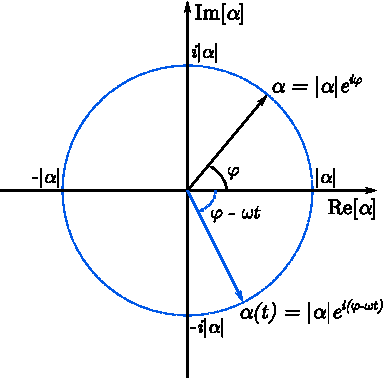
\includegraphics[width=0.85\linewidth]{images/alpha_tevol.pdf}
%    \def\svgwidth{0.85\linewidth}
%    \input{images/alpha_tevol_v2.pdf_tex}
%  \end{minipage}%
%  \begin{minipage}[t]{0.5\textwidth}
%    \vspace{10pt}
%    \captionof{figure}{Evolución temporal de un estado coherente. Si
%      inicialmente el sistema se encuentra en el estado coherente con autovalor
%      $\alpha = \abs{\alpha}e^{i\varphi}$, entonces a tiempo $t$ el sistema
%      pasa a estar en un estado coherente con autovalor $\alpha(t) = \alpha
%      e^{-i\wt} = \abs{\alpha} e^{i(\varphi - \wt)}$. Por lo tanto, $\alpha(t)$
%      rota en el plano complejo alrededor de una circunferencia de radio
%      $\abs{\alpha}$ en sentido horario con velocidad angular $\omega$.}
%    \label{fig:alpha_t}
%  \end{minipage}
%\end{figure}

\begin{figure}[tb]
  \centering
  \begin{minipage}{.5\textwidth}
    \centering
    \def\svgwidth{0.85\linewidth}
    \input{images/alpha_tevol_v2.pdf_tex}
  \end{minipage}%
  \begin{minipage}{.5\textwidth}
    \centering
    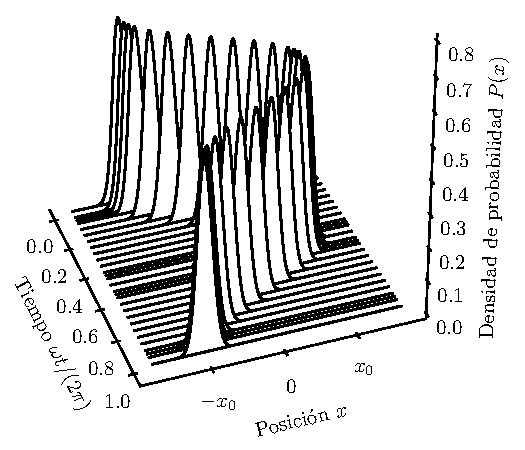
\includegraphics[width=\linewidth]{images/coherent_oscillation_3d.pdf}
  \end{minipage}
  \par
  \medskip
  \noindent
  \begin{minipage}[t]{.49\textwidth}
    \centering
    \captionof{figure}{Evolución temporal de un estado coherente. Si
      inicialmente el sistema se encuentra en el estado coherente con autovalor
      $\alpha = \abs{\alpha}e^{i\varphi}$, entonces a tiempo $t$ el sistema
      pasa a estar en un estado coherente con autovalor $\alpha(t) = \alpha
      e^{-i\wt} = \abs{\alpha} e^{i(\varphi - \wt)}$. Por lo tanto, $\alpha(t)$
      rota en el plano complejo alrededor de una circunferencia de radio
      $\abs{\alpha}$ en sentido horario con velocidad angular $\omega$.}
    \label{fig:alpha_t}
  \end{minipage}%
  \hfill
  \begin{minipage}[t]{.49\textwidth}
    \centering
    \captionof{figure}{Densidad de probabilidad de un estado coherente a
      distintos tiempo. A todo tiempo se tiene una densidad de probabilidad
      normal (de mínima incerteza) cuya forma no cambia sino que solamente
      se desplaza rígidamente, con el valor medio siguiendo exactamente la
      trayectoria de un oscilador clásico. Si inicialmente $\Im[\alpha] = 0$ y
      $\Re[\alpha] = x_0/\left(\xprefactsq\right)$, la posición $x_0$ actúa
      como punto de retorno del oscilador y el valor medio del paquete
      Gaussiano oscila armónicamente entre $x_0$ y $-x_0$.}
    \label{fig:coh_gauss_t}
  \end{minipage}
\end{figure}

\bigbreak

Como el estado del sistema es un estado coherente, calcular los valores medios
de posición y momento en función del tiempo es inmediato de las ecuaciones ya
antes encontradas en \eqref{eq:expval_x_alpha} y \eqref{eq:expval_p_alpha}
simplemente reemplazando $\alpha$ por $\alpha(t)$. Si el estado coherente
inicial es $\ket{\alpha}$ con $\alpha = \abs{\alpha}e^{i\varphi}$, entonces
$\alpha(t) = \abs{\alpha}e^{i(\varphi-\wt)}$ y por lo tanto los valores medios
son
\begin{align}
  \expval{x}(t) &= \xprefact\,2\Re[\alpha(t)] =
    \xprefact\,2\abs{\alpha}\cos(\varphi-\wt),
    \label{eq:expval_x_alpha_tevol} \\
  \expval{p}(t) &= \pprefact\,2\Im[\alpha(t)] =
    \pprefact\,2\abs{\alpha}\sin(\varphi-\wt).
    \label{eq:expval_p_alpha_tevol}
\end{align}

Notablemente, los valores medios de $x$ y $p$ oscilan armónicamente siguiendo
exactamente la trayectoria de un oscilador armónico clásico con posición
inicial $\xprefact 2\abs{\alpha}\cos\varphi = \xprefact 2\Re[\alpha]$ y momento
inicial $\pprefact 2\abs{\alpha}\sin\varphi = \pprefact 2\Im[\alpha]$.
Por otro lado, como las varianzas de $x$ y $p$ en un estado coherente no
dependen de $\alpha$, se mantienen constantes en el tiempo. Es más, como los
estados coherentes son todos paquetes Gaussianos de incerteza mínima, el estado
del sistema es a todo tiempo un paquete de onda Gaussiano de incerteza mínima.
En conclusión, como se muestra en un ejemplo en la figura
\ref{fig:coh_gauss_t}, la evolución de un oscilador armónico cuántico en un
estado coherente tiene una interpretación muy sencilla y que recuerda mucho a
un oscilador clásico: tenemos el sistema inicialmente en un estado Gaussiano
(i.e. una densidad de probabilidad normal en posición y momento) de incerteza
mínima y al evolucionar el tiempo la forma del paquete se mantiene constante,
simplemente variando su valor medio; además el valor medio de posición y
momento oscilan armónicamente siguiendo exactamente la trayectoria clásica.

\bigbreak

\TODO{rehacer evolución pero en Heisenberg}

% -----------------------------------------------------------------------------
\subsection{Problema 7 (Guía 5):
  Operador desplazamiento en el espacio de fases}
\label{exc:phase_despl_op}

En este problema introducimos el operador de desplazamiento en el espacio de
fases y vemos cómo se puede utilizar para construir estados coherentes
arbitrarios a partir del estado fundamental del oscilador armónico.

El operador de \emph{desplazamiento en el espacio de fases} $D(\alpha)$ se
define como
\begin{equation} \label{eq:def_phase_trans}
  D(\alpha) = e^{\alpha a^\dagger - \conj{\alpha}a}, \qquad\alpha\in\Complex.
\end{equation}

\bigbreak

En primer lugar nos piden verificar que el operador es unitario y que además
$D^{-1}(\alpha) = D(-\alpha)$. Para ello calculemos el adjunto de $D(\alpha)$
\begin{equation}
  \left(D(\alpha)\right)^\dagger = \left(e^{\alpha a^\dagger -
    \conj{\alpha}a}\right)^\dagger = e^{\left(\alpha a^\dagger -
    \conj{\alpha}a\right)^\dagger} = e^{\conj{\alpha} a - \alpha a^\dagger}
    = D(-\alpha).
\end{equation}
Falta ver que $D(-\alpha) = D^{-1}(\alpha)$. Efectivamente
\begin{equation}
  D(\alpha)D(-\alpha) =  e^{\alpha a^\dagger - \conj{\alpha}a} \;
    e^{-\left(\alpha a^\dagger - \conj{\alpha}a\right)} = 
    e^{\left(\alpha a^\dagger - \conj{\alpha}a\right) -\left(\alpha a^\dagger -
    \conj{\alpha}a\right)} = \Id.
\end{equation}
(\emph{CUIDADO}: recordemos que en general $e^Ae^B \neq e^{A+B}$; de hecho esto
es cierto solo en el caso en que $A$ y $B$ conmutan. En la cuenta anterior los
dos exponentes conmutan porque tenemos $B = -A$).

Por lo tanto, efectivamente tenemos que $D(\alpha)$ es unitario y $D(-\alpha)$
es la inversa.

\bigbreak

Antes de continuar analizando las propiedades de $D(\alpha)$ vale la pena
evaluar el operador para ciertos valores particulares de $\alpha$ para ver qué
se obtiene.

En primer lugar, para $\alpha$ real, es decir $\alpha = r$, $r \in \Reals$
tenemos
\begin{equation}
  D(r\in\Reals) = e^{ra^\dagger - ra} = e^{r\left(a^\dagger - a\right)} =
    e^{-i\frac{\sqrt{2}r}{\sqrt{\hbar m \omega}}p},
\end{equation}
donde $p$ es el operador de momento y usamos \eqref{eq:xp_aad} para escribir
$a^\dagger - a$ en términos de $p$. Por lo tanto $D(r\in\Reals)$ es simplemente
el operador de traslación (espacial).

En segundo lugar, para $\alpha$ imaginario puro, es decir $\alpha = ik$, $k \in
\Reals$ tenemos
\begin{equation}
  D(ik) = e^{ika^\dagger + ika} = e^{ik\left(a^\dagger + a\right)} =
    e^{i\frac{k\sqrt{2m\omega}}{\sqrt{\hbar}}x},
\end{equation}
donde $x$ es el operador posición y usamos \eqref{eq:xp_aad} para escribir
$a^\dagger + a$ en términos de $x$. Por lo tanto $D(ik)$, $k\in\Reals$ es
simplemente el operador de translación en el espacio de momentos.

En el caso más general, escribiendo $a$ y $a^\dagger$ en términos de $x$ y $p$
es fácil ver que el exponente de $D(\alpha)$ se puede escribir como una
combinación lineal de $x$ y $p$; lo cual se puede interpretar como una
combinación de una traslación en posición y en momento.

\bigbreak

\TODO{hacer esta cuenta.}

\bigbreak

Para los operadores de traslación espacial y de momento vale la regla de
composición $\mathcal{T}(a + b) = \mathcal{T}(a)\mathcal{T}(b)$. Para el
operador $D(\alpha)$ se tiene un resultado similar aunque, como veremos,
aparece una fase adicional. Queremos calcular
\begin{equation}
  D(\alpha)D(\beta) = e^{\alpha a^\dagger - \conj{\alpha}a} e^{\beta a^\dagger
    - \conj{\beta}a}.
\end{equation}
Para ello, usamos un resultado que demostramos en la guía de formalismo que
dice que si $A$ y $B$ son dos operadores que conmutan con su conmutador,
entonces
\begin{equation} \label{eq:expsum_comm}
  e^{A}e^{B} = e^{A + B + \comm{A}{B}/2}, \qquad\text{si }\comm{A}{\comm{A}{B}}
    = \comm{B}{\comm{A}{B}} = 0.
\end{equation}
Si tomamos $A = \left(\alpha a^\dagger - \conj{\alpha}a\right)$ y $B =
\left(\beta\ a^\dagger - \conj{\beta}a\right)$, entonces
\begin{equation}
  \comm{A}{B} = \comm{\alpha a^\dagger - \conj{\alpha}a}
    {\beta\ a^\dagger - \conj{\beta}a} = -\alpha\conj{\beta}\comm{a^\dagger}{a}
    - \conj{\alpha}\beta\comm{a}{a^\dagger} = \alpha\conj{\beta} -
    \conj{\alpha}\beta = 2i\Im(\alpha\conj{\beta}).
\end{equation}
Claramente $A$ y $B$ conmutan con su conmutador (pues es una constante) y
entonces
\begin{equation}
  D(\alpha)D(\beta) = e^{\left(\alpha a^\dagger - \conj{\alpha}a\right) +
    \left(\beta a^\dagger - \conj{\beta}a\right) + i\Im(\alpha\conj{\beta})}
    = D(\alpha + \beta)\,e^{i\Im(\alpha\conj{\beta})}.
\end{equation}

\bigbreak

Para comenzar a ver la utilidad del operador $D(\alpha)$, veamos cómo se
transforman los operadores $a$, $a^\dagger$, $x$ y $p$ ante esta transformación
unitaria. Esto es, para $a$ queremos calcular
\begin{equation}
  D^\dagger(\alpha)\,a\,D(\alpha),
\end{equation}
(y análogamente para $a^\dagger$, $x$ y $p$). Para ello usamos el siguiente
resultado que demostramos en la guía de formalismo: dados dos operadores $A$ y
$B$ cualesquiera, vale que
\begin{equation} \label{eq:hbc_lemma}
  e^A\,B\,e^{-A} = B + \comm{A}{B} + \frac{1}{2!}\comm{A}{\comm{A}{B}} +
  \frac{1}{3!}\comm{A}{\comm{A}{\comm{A}{B}}} + \dots
\end{equation}
Tomando $A = \left(\alpha a^\dagger - \conj{\alpha}a\right)$ y $B = a$ tenemos
\begin{equation}
  \comm{A}{B} = \comm{\alpha a^\dagger - \conj{\alpha}a}{a} =
    \alpha\comm{a^\dagger}{a} = \alpha\Id.
\end{equation}
Luego, como $\comm{A}{B}$ es una constante, todos los siguientes conmutadores
en \eqref{eq:hbc_lemma} son todos cero. Por lo tanto,
\begin{equation} \label{eq:a_D_transf}
  D^\dagger(\alpha)\,a\,D(\alpha) = a + \alpha\Id
\end{equation}
Es decir que el operador $a$ aparece ``trasladado'' en una cantidad $\alpha$.

Para $a^\dagger$ podemos proceder análogamente. Alternativamente, podemos notar
que como sabemos cómo transforma $a$ ya sabemos también como transforma
$a^\dagger$ sin necesidad de cuentas adicionales; efectivamente
\begin{equation}
  \left(D^\dagger(\alpha)\,a\,D(\alpha)\right)^\dagger = 
  D^\dagger(\alpha)\,a^\dagger\,{D^\dagger}^\dagger(\alpha) =
  D^\dagger(\alpha)\,a^\dagger\,D(\alpha).
\end{equation}
Luego,
\begin{equation} \label{eq:adagger_D_transf}
  D^\dagger(\alpha)\,a^\dagger\,D(\alpha) = 
  \left(D^\dagger(\alpha)\,a\,D(\alpha)\right)^\dagger = 
  \left(a + \alpha\Id\right)^\dagger = a^\dagger + \conj{\alpha}\Id.
\end{equation}
Análogamente, $a^\dagger$ se ``traslada'' en $\conj{\alpha}$.

Aún más interesante es usar \eqref{eq:a_D_transf} y \eqref{eq:adagger_D_transf}
junto con las expresiones de $x$ y $p$ en función de $a$ y $a^\dagger$ (ec.
\eqref{eq:xp_aad}) para calcular cómo se transforman los operadores $x$ y $p$.
Tenemos
\begin{align}
  D^\dagger(\alpha)\,x\,D(\alpha) &= \xprefact\left(
    D^\dagger(\alpha)\,a\,D(\alpha) + D^\dagger(\alpha)\,a^\dagger\,D(\alpha)
    \right) = \xprefact\left(a + \alpha + a^\dagger + \conj{\alpha}\right)
    \nonumber \\
  &= x + \xprefact 2\Re[\alpha], \label{eq:x_D_transf} \\
  D^\dagger(\alpha)\,p\,D(\alpha) &= -i\pprefact\left(
    D^\dagger(\alpha)\,a\,D(\alpha) - D^\dagger(\alpha)\,a^\dagger\,D(\alpha)
    \right) = -i\pprefact\left(a + \alpha - a^\dagger - \conj{\alpha}\right)
    \nonumber \\
  &= p + \pprefact 2\Im[\alpha], \label{eq:p_D_transf}
\end{align}
Por lo tanto, tanto el operador $x$ como $p$ quedan trasladados en cantidades
proporcionales a la parte real e imaginaria, respectivamente, de $\alpha$.

\bigbreak

En el inciso \textbf{(d)} nos piden mostrar una de las propiedades más
interesantes del operador $D(\alpha)$: si aplicamos $D(\alpha)$ al estado
fundamental del oscilador armónico obtenemos un estado coherente con autovalor
$\alpha$. Queremos calcular
\begin{equation} \label{eq:planteo_prob_D_0}
  a\,D(\alpha)\ket{0}.
\end{equation}
Vamos a calcular esto de dos formas distintas. Por un lado, podemos proceder
análogamente a como hicimos en la introducción del oscilador armónico y tratar
de conmutar $a$ con $D(\alpha)$ y ver que queda. La otra utiliza el resultado
\eqref{eq:a_D_transf} de cómo transforma $a$ ante $D(\alpha)$.

Hagamos primero esta segunda alternativa dado que en este caso es mucho más
rápida y sencilla. Queremos usar el resultado \eqref{eq:a_D_transf}. Para ello
multiplicamos \eqref{eq:planteo_prob_D_0} por $D(\alpha)D^\dagger(\alpha) =
\Id$. Tenemos
\begin{align}
  a\,D(\alpha)\ket{0} &= 
    \overbrace{D(\alpha)D^{\dagger}(\alpha)}^{\Id}\,a\,D(\alpha)\ket{0} = 
    D(\alpha)\underbrace{D^{\dagger}(\alpha)\,a\,D(\alpha)}_{a + \alpha}\ket{0}
    = \nonumber \\
  &= D(\alpha)\left(a + \alpha\right)\ket{0} =
    D(\alpha)\Big(\underbrace{a\ket{0}}_{0} + \alpha\ket{0}\Big) \nonumber \\
  &= \alpha\,D(\alpha)\ket{0}.
\end{align}
Por lo tanto, $D(\alpha)\ket{0}$ es autoestado de $a$ con autovalor $\alpha$,
es decir
\begin{equation}
  D(\alpha)\ket{0} = \ket{\alpha}.
\end{equation}

La otra forma de demostrar esto es, como dijimos antes, tratar de conmutar $a$
y $D(\alpha)$ en \eqref{eq:planteo_prob_D_0}. Tenemos
\begin{equation} \label{eq:planteo_prob_D_0_eq2}
  a\,D(\alpha)\ket{0} = \left(D(\alpha)\,a + \comm{a}{D(\alpha)}\right)\ket{0}
  = D(\alpha)\,\underbrace{a\ket{0}}_{0} + \comm{a}{D(\alpha)}\ket{0}
  = \comm{a}{D(\alpha)}\ket{0}.
\end{equation}
Tenemos que entonces calcular $\comm{a}{D(\alpha)}$. Para ello usamos un
resultado que demostramos en la guía de formalismo: sean $A$ y $B$ operadores
tales que $B$ conmuta con $\comm{A}{B}$ y $f$ una función desarrollable en
serie de potencias, entonces
\begin{equation}
  \comm{A}{f(B)} = \dv{f(B)}{B} \,\comm{A}{B}.
\end{equation}
Tomemos $A = a$, $B = \left(\alpha a^\dagger - \conj{\alpha}a\right)$ y
$f(\cdot) = \exp(\cdot)$. Tenemos
\begin{equation}
  \comm{A}{B} = \comm{a}{\alpha a^\dagger - \conj{\alpha}a} =
    \alpha\comm{a}{a^\dagger} = \alpha.
\end{equation}
Claramente, $B$ conmuta con $\comm{A}{B}$. Además, por la elección de función
$f$ tenemos $f' = f$. Entonces
\begin{equation}
  \comm{a}{D(\alpha)} = D(\alpha)\,\alpha = \alpha\,D(\alpha)
\end{equation}
Finalmente, reemplazando en \eqref{eq:planteo_prob_D_0_eq2} tenemos
\begin{equation}
  a\,D(\alpha)\ket{0} = \comm{a}{D(\alpha)}\ket{0} = \alpha\,D(\alpha)\ket{0}.
\end{equation}

\bigbreak

En conclusión mostramos que aplicar el operador de desplazamiento en el espacio
de fases al estado fundamental del oscilador armónico nos da un estado
coherente. Como además antes mostramos que el operador $D(\alpha)$ se puede
pensar como una composición de una traslación espacial y una en momento,
entonces el estado coherente $\ket{\alpha}$ no es más que el estado fundamental
del oscilador armónico trasladado espacialmente y en momento.

Esto nos permite, por ejemplo, ver una forma sencilla de crear un estado
coherente, que se muestra esquematizada en la figura
\ref{fig:coh_gen_pot_onoff}. Supongamos que inicialmente tenemos un potencial
armónico y el sistema se encuentra en el estado fundamental, $\ket{\psi} =
\ket{0}$. Luego, muy rápidamente apagamos el potencial armónico original y
prendemos uno nuevo, con la misma frecuencia, pero cuyo punto de equilibrio
está corrido una distancia $x_0$. Por lo tanto, desde el punto de vista del
nuevo potencial, el estado del sistema es el estado fundamental, pero
trasladado espacialmente en $-x_0$, es decir que $\ket{\psi'} =
D(-x_0)\ket{0}$. Por lo tanto, tenemos un estado coherente y el estado del
sistema comenzará a oscilar armónicamente, tal como vimos antes en la figura
\ref{fig:coh_gauss_t}.

\begin{figure}[tb]
  \centering
  \def\svgwidth{0.85\linewidth}
  \input{images/pot_onoff.pdf_tex}
  \captionof{figure}{Posible forma de generar un estado coherente.
    Inicialmente tenemos un potencial armónico y el sistema se encuentra en el
    estado fundamental ($\alpha = 0$). Luego, rápidamente apagamos el potencial
    y lo volvemos a encender, con misma frecuencia, pero trasladado una
    distancia $x_0$ respecto de la posición de equilibrio original. Por lo
    tanto, para el nuevo potencial, la partícula se encuentra en el estado
    fundamental trasladado una distancia $-x_0$; es decir que $\ket{\psi} =
    D(-x_0)\ket{0} = \ket{\alpha' = -x_0}$. Por lo tanto, el sistema se
    encuentra en un estado coherente y comenzará a oscilar armónicamente, tal
    como vimos antes en la figura \ref{fig:coh_gauss_t}.}
  \label{fig:coh_gen_pot_onoff}
\end{figure}

Más adelante, en el problema del oscilador forzado (\ref{exc:forcedho}) veremos
otro método para generar estados coherentes de un oscilador.

\bigbreak

Por último, vale la pena notar que el operador $D(\alpha)$ se puede reescribir
de otra forma, particularmente útil para ciertos cálculos. Vamos a utilizar la
propiedad \eqref{eq:expsum_comm} de la guía de formalismo, tomando $A = \alpha
a^\dagger$ y $B = -\conj{\alpha}a$. En tal caso tenemos
\begin{equation}
  \comm{A}{B} = \comm{\alpha a^\dagger}{-\conj{\alpha}a} =
  -\abs{\alpha}^2\comm{a^\dagger}{a} = \abs{\alpha}^2.
\end{equation}
Claramente $A$ y $B$ conmutan con $\comm{A}{B}$ dado que este último es una
constante. Luego,
\begin{equation}
  D(\alpha) = e^{-\abs{\alpha}^2/2}\,e^{\alpha a^\dagger}\,e^{-\conj{\alpha}a}.
\end{equation}
A esta forma de escribir $D(\alpha)$ se la suele llamar \emph{descomposición en
orden normal} de $D(\alpha)$.

Notemos que si aplicamos $D(\alpha)$ escrito de esta forma al estado $\ket{0}$
para obtener $\ket{\alpha}$ tenemos
\begin{equation}
  \ket{\alpha} = D(\alpha)\ket{0} = 
  e^{-\abs{\alpha}^2/2}\,e^{\alpha a^\dagger}\,e^{-\conj{\alpha}a} \ket{0} =
  e^{-\abs{\alpha}^2/2}\,e^{\alpha a^\dagger} \ket{0},
\end{equation}
donde en la última igualdad usamos que $a\ket{0} = 0$ y, por lo tanto,
$e^{-\conj{\alpha}a}\ket{0} = \ket{0}$. Notemos además que si expandimos
$e^{\alpha a^\dagger}$ en series de potencias tenemos
\begin{equation}
  \ket{\alpha} = 
  e^{-\abs{\alpha}^2/2}\,\sum_{n=0}^{\infty} \frac{\left(\alpha
  a^\dagger\right)^n}{n!} \ket{0} =
  e^{-\abs{\alpha}^2/2}\,\sum_{n=0}^{\infty} \frac{\alpha^n}{\sqrt{n!}}
  \underbrace{\frac{{a^\dagger}^n}{\sqrt{n!}} \ket{0}}_{\ket{n}} =
  e^{-\abs{\alpha}^2/2}\,\sum_{n=0}^{\infty} \frac{\alpha^n}{\sqrt{n!}}
  \ket{n}.
\end{equation}
Esta es justamente la expansión del estado coherente $\ket{\alpha}$ en la base
$\set{\ket{n}}$ que calculamos en \eqref{eq:alpha_n_basis}.

\bigbreak

\TODO{observar que si H tal que D = U => me permite generar estados coherentes}

% -----------------------------------------------------------------------------
\subsection{Curiosidad: ¿Autoestados del operador de creación?}

En las secciones anteriores estudiamos con cierto detalle los estados
coherentes, que son autoestados del operador de aniquilación y exhiben una gran
variedad de propiedades que los hace muy similares al estado de un oscilador
armónico clásico. Una pregunta que puede naturalmente surgir es: ¿qué pasa con
los autoestados del operador de creación? ¿qué propiedades tienen? ¿tienen
alguna interpretación física? Como veremos, la respuesta es muy sencilla, en
cuanto \emph{no existen} autoestados de $a^\dagger$.

\bigbreak

Supongamos que existe un estado $\ket{\psi}$ que es autoestado de $a^\dagger$
con autovalor $\lambda$,
\begin{equation}
  a^\dagger\ket{\psi} = \lambda\ket{\psi}.
\end{equation}
Por otro lado, expandiendo $\ket{\psi}$ en la base $\set{\ket{n}}$ y aplicando
$a^\dagger$ tenemos
\begin{align}
  \ket{\psi} &= \sum_{n=0}^\infty c_n\ket{n}, \\
  a^\dagger\ket{\psi} &= a^\dagger\left(\sum_{n=0}^\infty c_n\ket{n}\right) =
    \sum_{n=0}^\infty c_na^\dagger\ket{n} = \sum_{n=0}^\infty
    c_n\sqrt{n+1}\ket{n+1} = \sum_{n=1}^\infty c_{n-1}\sqrt{n}\ket{n}.
\end{align}
Entonces, necesitamos que valga
\begin{equation}
  \lambda\,\sum_{n=0}^\infty c_n\ket{n} = \sum_{n=1}^\infty
    c_{n-1}\sqrt{n}\ket{n}.
\end{equation}
Como $\set{\ket{n}}$ es una base ortonormal, esta igualdad es cierta si y solo
si la igualdad vale coeficiente a coeficiente de la expansión, $\lambda\,c_n =
c_{n-1}\sqrt{n}$ (análogamente, proyectando ambos lados de la igualdad sobre
$\bra{n}$ tenemos la igualdad coeficiente a coeficiente). En particular,
notemos que la suma del término a la izquierda comienza en $\ket{0}$ ($n = 0$),
mientras que en el término de la derecha el estado $\ket{0}$ no aparece; esto
implica que $c_0 = 0$. En resumen, tenemos
\begin{align}
  c_0 &= 0, \\
  \lambda\,c_n &= c_{n-1}\sqrt{n}, \quad\forall n \geq 1.
\end{align}
Claramente, esta relación de recurrencia tiene una única solución que es $c_n =
0$, $\forall n$. Por lo tanto, $\ket{\psi} = 0$ y $a^\dagger$ no tiene ningún
autovector.

\bigbreak

Aquí vemos otra peculiaridad de trabajar con operador no normales a diferencia
de los operadores normales con los que estamos acostumbrados. Mientras que $a$
sí tiene autoestados (y de hecho forman una base, aunque no ortogonal), el
operador $a^\dagger$ en cambio no admite ningún autoestado.

% =============================================================================
\section{Otros Potenciales}

La idea de esta sección de la práctica es estudiar algunos potenciales que,
aunque no son osciladores armónicos simples, se pueden reducir a problemas
equivalentes de osciladores o se pueden trabajar con las herramientas aplicadas
al tratamiento del oscilador común.

% -----------------------------------------------------------------------------
\subsection{Problema 9 (Guía 5): El oscilador armónico forzado}
\label{exc:forcedho}

La idea de este problema es estudiar una modificación relativamente sencilla
del oscilador armónico ordinario, el oscilador armónico forzado por una fuerza
constante $F$. El Hamiltoniano del problema es
\begin{equation}
  H = \frac{p^2}{2m} + \frac{m\omega^2}{2}x^2 - Fx
    = H_0 - Fx
\end{equation}
donde $H_0 = \frac{p^2}{2m} + \frac{m\omega^2}{2}x^2$ es el Hamiltoniano de un
oscilador armónico ordinario y $F$ es una constante real. En realizaciones
típicas de este Hamiltoniano, la partícula sometida al potencial armónico es
una partícula cargada y la fuerza $F = qE$ se debe a una fuerza electrostática
externa que se aplica.

Clásicamente, cuando uno agrega una fuerza constante a un partícula sometida a
un potencial armónico, el único efecto es cambiar la posición de equilibrio del
sistema. Veremos que en el caso cuántico sucede básicamente lo mismo.
Notablemente, como veremos, esto nos da un método para generar estados
coherentes del oscilador ordinario.

\subsubsection{Reescritura del Hamiltoniano en términos de operadores creación
  y aniquilación}
En el primer inciso del problema nos piden escribir el Hamiltoniano en función
de los operadores $a$ y $a^\dagger$ del oscilador ordinario (ec.
\eqref{eq:def_a_adagger}). La cuenta es bastante directa y no trae mayores
dificultades. Simplemente usamos cómo se escriben $x$ y $p$ en función de $a$ y
$a^\dagger$ (ec. \eqref{eq:xp_aad}) y luego reemplazamos en el Hamiltoniano. El
término $H_0$ nos dará en Hamiltoniano del oscilador ordinario en términos de
$a$ y $a^\dagger$ y el término nuevo es simplemente proporcional a $x$. Por lo
tanto
\begin{equation}
  H = \hbar\omega\left(a^\dagger a + \frac{1}{2}\right) -
    F\xprefact\left(a^\dagger + a\right)
\end{equation}

\subsubsection{Valor medio y varianza de energía en autoestados del operador
  número}
En segundo lugar vamos a calcular los valores medios $\bra{n}H\ket{n}$ y
$\bra{n}H^2\ket{n}$ y con ellos la varianza de la energía en los autoestados
del operador de número $N$. El primero de estos valores medios sale
inmediatamente haciendo uso de los resultados ya conocidos del oscilador
armónico ordinario (ver problema \ref{sec:expval_ketn})
\begin{align}
  \bra{n}x\ket{n} &= 0 \\
  \bra{n}p\ket{n} &= 0 \\
  \bra{n}x^2\ket{n} &= (2n + 1)\frac{\hbar}{2m\omega} \\
  \bra{n}p^2\ket{n} &= (2n + 1)\frac{m\omega\hbar}{2}
\end{align}
Luego,
\begin{align}
  \bra{n}H\ket{n} &= \frac{1}{2m}\bra{n}p^2\ket{n} +
    \frac{m\omega^2}{2}\bra{n}x^2\ket{n} - F\bra{n}x\ket{n} \\
  &= \frac{1}{2m}(2n + 1)\frac{m\omega\hbar}{2} +
    \frac{m\omega^2}{2}(2n + 1)\frac{\hbar}{2m\omega} - F\cdot 0 \\
  &= \frac{\hbar\omega}{2}(2n + 1) = \hbar\omega\left(n + \frac{1}{2}\right)
\end{align}

Para el valor medio de $H^2$ notemos que la ayuda que recién usamos nos dice
que $\bra{n}x\ket{n} = 0$, o, lo que es lo mismo, $\bra{n}(a + a^\dagger)
\ket{n} = 0$. Por lo tanto, al expandir la expresión de $H^2$, nos conviene
mantener los términos con $(a + a^\dagger)$ juntos y no expandir los
respectivos cuadrados. Además, notemos que en $H = H_0 - F \xprefact
\left(a^\dagger + a\right)$, el primer término, $H_0 = \hbar\omega(a^\dagger a
+ 1/2)$, tiene a los kets $\ket{n}$ como autoestados, es decir $H_0\ket{n} =
\hbar\omega(n + 1/2)\ket{n}$. Esto va simplificar significativamente el cálculo
de los valores medios en un estado $\ket{n}$. Por este motivo al expandir $H^2$
también nos conviene mantener el término $H_0$ junto y no expandir los términos
de adentro. Haciendo esto tenemos
\begin{align}
  \bra{n}H^2\ket{n} &= \bra{n}\left(H_0 - F \xprefact (a^\dagger + a)\right)^2
    \ket{n} \\
  &= \bra{n}\left(H_0^2 + F^2\xprefactsq(a^\dagger + a)^2 - F\xprefact
    (H_0(a^\dagger + a) + (a^\dagger + a)H_0)\right)\ket{n} \\
  &= \bra{n}H_0^2\ket{n} + \bra{n}F^2\xprefactsq (a^\dagger + a)^2\ket{n} - F
    \xprefact \left(\bra{n}H_0(a^\dagger + a)\ket{n} + \bra{n}
    (a^\dagger + a)H_0\ket{n}\right) \\
  &= (\hbar\omega)^2\left(n + \frac{1}{2}\right)^2 + F^2(2n + 1)
    \xprefactsq - F\xprefact\hbar\omega\left(n + \frac{1}{2}\right)\left(
    \bra{n}(a^\dagger + a)\ket{n} + \bra{n}(a^\dagger + a)\ket{n}\right) \\
  &= (\hbar\omega)^2\left(n + \frac{1}{2}\right)^2 + F^2(2n + 1)
    \frac{\hbar}{2m\omega}
\end{align}
donde usamos que como $H_0$ es hermítico y $\ket{n}$ es autoestado, entonces,
$H_0\ket{n} = \hbar\omega(n + 1/2)\ket{n}$ y $\bra{n}H_0 = \hbar\omega(n +
1/2)\bra{n}$ (esta segunda relación se obtiene de la primera tomando el adjunto
de ambos miembros de la igualdad y usando que $H_0$ es hermítico) y además
usamos los resultados de $\bra{n}x\ket{n}$ y $\bra{n}x^2\ket{n}$ escritos en
términos de $a$ y $a^\dagger$.

Luego, la varianza queda
\begin{equation}
  \Var(H^2) = \expval{H^2} - \expval{H}^2 = F^2\xprefactsq\left(2n + 1\right).
\end{equation}

\bigbreak

Finalmente, el inciso pregunta si la base de autoestados de $H_0$,
$\set{\ket{n}}$, puede coincidir con la de $H$. Hay distintas formas de
contestar la pregunta, todas perfectamente válidas. Una opción es aplicar $H$
sobre un $\ket{n}$ y mostrar que no queda algo proporcional a $\ket{n}$ (salvo
que $F = 0$). Por otro lado, se puede calcular el conmutador $\comm{H}{N}$,
con $N = a^\dagger a$ el operador de número del oscilador ordinario, y
mostraron que no conmutan. Alternativamente, otra respuesta válida consiste en
notar que según el resultado recién obtenido, la varianza de la energía es
distinta de cero. Por lo tanto, $\ket{n}$ no puede ser autoestado de $H$
porque la varianza de un observable es cero en un estado si y sólo si el estado
es autoestado del observable (y por lo tanto el estado tiene un valor del
observable bien definido).

\subsubsection{Autoestados del oscilador forzado}
Ahora vamos a encontrar la base de autoestados del oscilador forzado. Para
ello, el inciso \textbf{(c)} del problema nos propone una forma particular de
mostrarlo (si buscan el problema del oscilador forzado online, seguro van a
encontrar varias otras formas de resolver el problema, como por ejemplo
redefinir un nuevo operador posición, y otras; la forma aquí presentada apunta
fundamentalmente a resaltar ciertas propiedades del estado que van a ser
esenciales para luego hacer la conexión con los estados coherentes del
oscilador ordinario).

Dada la base $\set{\ket{n}}$ del operador número (y del oscilador ordinario),
definimos una nueva base trasladada en posición en una distancia $\ell$ como
\begin{equation}
  \ket{n,\ell} = e^{-ip\ell/\hbar}\ket{n}.
\end{equation}
(recordemos que efectivamente $e^{-ip\ell/\hbar}$ es el operador de traslación
espacial en una distancia $\ell$). La idea es buscar el valor de $\ell$ tal que
$\ket{n,\ell}$ son autoestados del Hamiltoniano forzado $H$, es decir
\begin{equation}
  H\ket{n,\ell} = E\ket{n,\ell}.
\end{equation}

La dificultad pasa, por empezar, porque no es trivial ver cómo opera
$e^{-ip\ell/\hbar}$ sobre un ket $\ket{n}$ cualquiera en términos de los
elementos de la base $\set{\ket{n}}$ y, por lo tanto, tampoco ver cómo
opera $H$ sobre $\ket{n,\ell}$. Vamos a ver dos posibles caminos para resolver
este inciso. Antes de pasar a la resolución vale la pena recordar que este
problema es muy parecido a uno de los incisos que resolvimos en el problema
\ref{exc:phase_despl_op}, en que se pedía demostrar que $aD(\alpha)\ket{0} =
\alpha D(\alpha)\ket{0}$. Efectivamente, las dos formas que para resolver el
problema ahora, son análogas a las dos formas que usamos antes para esa otra
pregunta.

Veamos primero una forma de calcular los deseado utilizando el lema de la
fórmula de Baker-–Campbell-–Hausdorff (BCH), que nos decía cómo calcular
$e^ABe^{-A}$ para dos operadores $A$ y $B$ cualesquiera (ec.
\eqref{eq:hbc_lemma}).
Queremos calcular
\begin{equation}
  H\ket{n,\ell} = He^{-ip\ell/\hbar}\ket{n}.
\end{equation}
Entonces para usar la fórmula BCH, multiplicamos a izquierda por $\Id =
e^{-ip\ell/\hbar}e^{ip\ell/\hbar}$. Tenemos,
\begin{equation}
  He^{-ip\ell/\hbar}\ket{n} =
  e^{-ip\ell/\hbar}e^{ip\ell/\hbar}He^{-ip\ell/\hbar}\ket{n},
\end{equation}
y entonces podemos aplicar la fórmula BCH a
\begin{equation}
  e^{ip\ell/\hbar}He^{-ip\ell/\hbar}.
\end{equation}
Antes de proceder a calcular, notemos otro razonamiento con el cuál podemos
llegar a plantear el mismo cálculo. Si escribimos explícitamente la condición
de autoestado tenemos
\begin{equation}
  H\ket{n \ell} = E\ket{n,\ell}.
\end{equation}
Usando la definición de $\ket{n ,\ell}$ esto es equivalente a
\begin{equation}
  He^{-ip\ell/\hbar}\ket{n} = Ee^{-ip\ell/\hbar}\ket{n}.
\end{equation}
La expresión a la izquierda es casi lo que aparece en la fórmula BCH,
salvo que falta una exponencial $e^{+ip\ell/\hbar}$ a la izquierda de $H$. Para
hacer que aparezca podemos multiplicar a ambos miembros de la igualdad por este
operador obteniendo
\begin{equation}
  e^{ip\ell/\hbar}He^{-ip\ell/\hbar}\ket{n} =
  e^{ip\ell/\hbar}Ee^{-ip\ell/\hbar}\ket{n} = E\ket{n},
\end{equation}
donde usamos que $e^{ip\ell/\hbar} = \left(e^{-ip\ell/\hbar}\right)^{-1}$.
Notemos que esta igualdad es simplemente una ecuación de autovalores para el
operador Hamiltoniano transformado $e^{ip\ell/\hbar}He^{-ip\ell/\hbar}$, donde
lo que buscamos es $\ell$ tal que los kets $\ket{n}$ sean los autoestados.

Ahora sí, escribamos cómo queda el operador $H$ transformado,
$e^{ip\ell/\hbar}He^{-ip\ell/\hbar}$, usando BCH (ec. \eqref{eq:hbc_lemma}).
\begin{equation}
  e^{ip\ell/\hbar}He^{-ip\ell/\hbar} = H + \comm{ip\ell/\hbar}{H} +
  \frac{1}{2}\comm{ip\ell/\hbar}{\comm{ip\ell/\hbar}{H}} +
  \frac{1}{3!}\comm{ip\ell/\hbar}{\comm{ip\ell/\hbar}{\comm{ip\ell/\hbar}{H}}}
  + \cdots
\end{equation}
Para el primer conmutador tenemos
\begin{align}
  \comm{ip\ell/\hbar}{H} &= \frac{i\ell}{\hbar}\comm{p}{\frac{p^2}{2m} +
    \frac{m\omega^2}{2}x^2 - Fx} =
    \frac{i\ell}{\hbar}\comm{p}{\frac{m\omega^2}{2}x^2 - Fx} \\
  &= \frac{i\ell}{\hbar}\left(\frac{m\omega^2}{2}\comm{p}{x^2} -
    F\comm{p}{x}\right) = \frac{i\ell}{\hbar}\left(\frac{m\omega^2}{2}
    (-2i\hbar x) - F(-i\hbar\Id)\right). \\
  &= \ell m\omega^2x -\ell F\Id,
\end{align}
donde usamos que $\comm{p}{G(x)} = -i\hbar\dv{G}{x}$.
Para el segundo conmutador tenemos
\begin{align}
  \comm{ip\ell\hbar}{\comm{ip\ell/\hbar}{H}}
  &= \frac{i\ell}{\hbar}\comm{p}{\ell m\omega^2x - \ell F\Id} =
    \frac{i\ell}{\hbar}\comm{p}{\ell m\omega^2x} \\
  &= \frac{i\ell^2m\omega^2}{\hbar}\comm{p}{x}
    = \frac{i\ell^2m\omega^2}{\hbar}(-i\hbar\Id) \\
  &= \ell^2m\omega^2\Id
\end{align}
Como este conmutador es proporcional a la identidad, entonces todos los
siguientes términos en la serie se anulan. Finalmente
\begin{equation}
  e^{ip\ell/\hbar}He^{-ip\ell/\hbar} = H + \ell m\omega^2x -\ell F\Id +
  \frac{\ell^2m\omega^2}{2}\Id
\end{equation}
Notemos que el Hamiltoniano transformado nos quedó escrito en términos de
operadores $x$, $p$ (e identidades) y por lo tanto también en términos de $a$ y
$a^\dagger$. Por lo tanto, podemos calcular cómo opera este operador sobre
$\ket{n}$ y así resolver la ecuación de autovalores. Para hacer esto de forma
sencilla, recordemos que $H = H_0 - Fx$ y reescribamos primero el operador
Hamiltoniano transformado de la forma
\begin{equation}
  e^{ip\ell/\hbar}He^{-ip\ell/\hbar} = H_0 + \left(\frac{\ell^2m\omega^2}{2} -
  \ell F\right)\Id + (\ell m\omega^2 - F)x
\end{equation}
Notemos que para los primeros dos términos (el Hamiltoniano del oscilador
ordinario $H_0$ y un operador proporcional a la identidad) ya se satisface que
$\ket{n}$ es autoestado; solamente hace falta que también valga para el término
proporcional a $x$. Tenemos
\begin{align}
  e^{ip\ell/\hbar}He^{-ip\ell/\hbar}\ket{n} &= \left(H_0 +
    \left(\frac{\ell^2m\omega^2}{2} - \ell F\right)\Id + (\ell m\omega^2 -
    F)x\right)\ket{n} \\
  &= \left(\hbar\omega\left(n + \frac{1}{2}\right) +
    \left(\frac{\ell^2m\omega^2}{2} - \ell F\right)\right)\ket{n} + (\ell
     m\omega^2 - F)x\ket{n} \\
  &= \left(\hbar\omega\left(n + \frac{1}{2}\right) +
    \left(\frac{\ell^2m\omega^2}{2} - \ell F\right)\right)\ket{n} + (\ell
    m\omega^2 - F) \xprefact(a^\dagger + a)\ket{n} \\
  &= \left(\hbar\omega\left(n + \frac{1}{2}\right) +
    \left(\frac{\ell^2m\omega^2}{2} - \ell F\right)\right)\ket{n} + (\ell
    m\omega^2 - F) \xprefact\left(\sqrt{n+1}\ket{n+1} +
    \sqrt{n}\ket{n-1}\right) \\
  &= E\ket{n}.
\end{align}
Notemos que $\set{\ket{n}}$ es una base ortonormal, es decir que los estados
$\ket{n}$ son todos linealmente independientes entre sí. Por lo tanto, la única
forma de que $\ket{n}$ sea autoestado es que los términos proporcionales a
$\ket{n+1}$ y $\ket{n-1}$ se anulen. Esto se tiene sólo si
\begin{equation}
  \ell m\omega^2 - F = 0 \;\implies\;
  \ell = \frac{F}{m\omega^2}.
\end{equation}
En tal caso, la energía correspondiente es todo el término que queda
multiplicando a $\ket{n}$:
\begin{equation}
  E_{n,\ell} = \hbar\omega\left(n + \frac{1}{2}\right) +
    \frac{\ell^2m\omega^2}{2} - \ell F = \hbar\omega\left(n +
    \frac{1}{2}\right) - \frac{F^2}{2m\omega^2},
\end{equation}
donde usamos que $\ell = F / (m\omega^2)$.

\bigbreak

Veamos ahora el otro posible camino para calcular el valor de $\ell$ tal que
$\ket{n,\ell}$ es autoestado de $H$. Partamos nuevamente de la ecuación de
autoestados inicial
\begin{equation}
  H\ket{n,\ell} = He^{-ip\ell/\hbar}\ket{n} = Ee^{-ip\ell/\hbar}\ket{n}.
\end{equation}
Como dijimos antes, no sabemos exactamente cómo escribir la acción de
$e^{-ip\ell/\hbar}$ sobre $\ket{n}$ en términos de los estados de la base
$\set{\ket{n}}$. Sin embargo, sí sabemos cómo actúa $H$ (pues lo tenemos
escrito en términos de $a$ y $a^\dagger$). Por lo tanto, podemos tratar de
conmutarlos, teniendo en cuenta cuanto vale en conmutador
\begin{equation}
  He^{-ip\ell/\hbar} = e^{-ip\ell/\hbar}H + \comm{H}{e^{-ip\ell/\hbar}}.
\end{equation}
La dificultad ahora es calcular el conmutador y ver si nos queda algo que
podemos aplicar sobre $\ket{n}$ de forma sencilla. Tenemos
\begin{align}
  \comm{H}{e^{-ip\ell/\hbar}} &= \comm{\frac{p^2}{2m} +
    \frac{m\omega^2}{2}x^2 - Fx}{e^{-ip\ell/\hbar}} =
    \comm{\frac{m\omega^2}{2}x^2 - Fx}{e^{-ip\ell/\hbar}} \\
  &= \frac{m\omega^2}{2}\comm{x^2}{e^{-ip\ell/\hbar}} -
    F\comm{x}{e^{-ip\ell/\hbar}}.
\end{align}

Para calcular estos conmutadores usamos un resultado que demostramos en la guía
de formalismo: sean $A$ y $B$ operadores tales que $B$ conmuta con
$\comm{A}{B}$ y $f$ una función desarrollable en serie de potencias, entonces
\begin{equation}
  \comm{A}{f(B)} = \dv{f(B)}{B} \,\comm{A}{B}.
\end{equation}

Para el segundo de los conmutadores, $\comm{x}{e^{-ip\ell/\hbar}}$ esta fórmula
se puede aplicar directamente puesto que $\comm{x}{p} = i\hbar$ y se satisface
la condición. Por lo tanto,
\begin{align}
  \comm{x}{e^{-ip\ell/\hbar}} &= -\frac{i\ell}{\hbar} e^{-ip\ell/\hbar}
    \comm{x}{p} = -\frac{i\ell}{\hbar} e^{-ip\ell/\hbar} (i\hbar) \\
  &= \ell e^{-ip\ell/\hbar}.
\end{align}

Para el primer conmutador, $\comm{x^2}{e^{-ip\ell/\hbar}}$, en cambio, como
$\comm{x^2}{p} = 2i\hbar x$, entonces no se satisface la condición de que $p$
conmute con el conmutador de $\comm{x^2}{p}$ para poder aplicar la fórmula.
Sin embargo, notemos que podemos usar otra propiedad vista en guías anteriores,
sobre el conmutador con el producto de operadores, $\comm{AB}{C} = \comm{A}{C}B
+ A\comm{B}{C}$, para reescribir el conmutador contra $x^2$ en términos de
conmutadores contra $x$, para los cuales sí vale la fórmula. Concretamente
\begin{align}
  \comm{x^2}{e^{-ip\ell/\hbar}} &= 
  \comm{x}{e^{-ip\ell/\hbar}}x + x\comm{x}{e^{-ip\ell/\hbar}} \\
  &= \ell e^{-ip\ell/\hbar}x + x\ell e^{-ip\ell/\hbar},
\end{align}
donde en la última igualdad notamos que vuelven a aparecer los conmutadores
ya antes calculados. Recordemos que todo esto es útil si podemos escribir los
operadores con las traslaciones a la izquierda y operadores que sabemos cómo
actúan sobre $\ket{n}$ a la derecha. Por lo tanto habría que conmutar de nuevo
el segundo término,
\begin{align}
  x e^{-ip\ell/\hbar} &= e^{-ip\ell/\hbar}x + \comm{x}{e^{-ip\ell/\hbar}} \\
  &= e^{-ip\ell/\hbar}x + \ell e^{-ip\ell/\hbar}.
\end{align}

Finalmente
\begin{align}
  \comm{H}{e^{-ip\ell/\hbar}} &=
    \frac{m\omega^2}{2}\comm{x^2}{e^{-ip\ell/\hbar}} -
    F\comm{x}{e^{-ip\ell/\hbar}} \\
  &= \frac{m\omega^2}{2} e^{-ip\ell/\hbar}\left(2\ell x  + \ell^2\right) -
    F\ell e^{-ip\ell/\hbar},
\end{align}
y entonces
\begin{align}
  He^{-ip\ell/\hbar} &= e^{-ip\ell/\hbar}H + \frac{m\omega^2}{2}
    e^{-ip\ell/\hbar}\left(2\ell x  + \ell^2\right) - F\ell e^{-ip\ell/\hbar}
    \\
  &= e^{-ip\ell/\hbar}\left(H + \frac{m\omega^2}{2} \left(2\ell x  +
    \ell^2\right) - F\ell\right).
\end{align}
Nuevamente agrupamos los términos proporcionales a $x$ y la resolución sigue
exactamente como en el caso anterior.

\bigbreak

Notemos el resultado obtenido en este inciso tiene una interpretación muy
sencilla. Demostramos que los autoestado del Hamiltoniano con un forzado
constante son los autoestados del oscilador ordinario trasladados en una
distancia $\ell = F / (m\omega^2)$. Recordemos que en mecánica clásica cuando
tenemos un oscilador con un forzado constante (piensen por ejemplo en el típico
problema de Física 2 de un resorte colgado del techo en el cuál se tiene en
cuenta la fuerza gravitatoria) el efecto que se tiene es justamente un simple
corrimiento del punto de equilibrio del sistema. Es más, si escriben las
ecuaciones de movimiento clásicas e imponen $\ddot{x} = 0$, van a obtener que
el corrimiento es justamente en una distancia $F / (m\omega^2)$. Todo esto es
completamente análogo a los resultados aquí obtenidos.

\subsubsection{El estado fundamental del oscilador forzado como estado
  coherente}
El inciso \textbf{(d)} es muy sencillo en términos de cálculos y consiste
simplemente en notar, como bien indica el enunciado, que todo estado coherente
$\ket{\alpha}$ se escribe como
\begin{equation}
  \ket{\alpha} = D(\alpha)\ket{0} = e^{\alpha a^\dagger - \alpha^* a}\ket{0}.
\end{equation}
donde $D(\alpha)$ es el operador desplazamiento en el espacio de fases (como
vimos bien en detalle en el problema \ref{exc:phase_despl_op}).
De las definiciones del inciso anterior tenemos que el estado fundamental del
oscilador forzado es
\begin{equation}
  \ket{0,\ell} = e^{-ip\ell/\hbar}\ket{0}.
\end{equation}
Por lo tanto, si reescribimos $p$ en función de $a$ y $a^\dagger$ (ver ec.
\eqref{eq:xp_aad}) tenemos
\begin{equation}
  \ket{0,\ell} = e^{\ell\sqrt{\frac{m\omega}{2\hbar}}(a^\dagger - a)}\ket{0}.
\end{equation}
Por lo tanto, el estado $\ket{0, \ell}$ es un estado coherente con autovalor
$\alpha = \ell\sqrt{\frac{m\omega}{2\hbar}}$ (efectivamente, en el problema
\ref{exc:phase_despl_op} mostramos que el operador de desplazamiento en el
espacio de fases $D(\alpha)$ evaluado en un $\alpha$ real no es más que el
operador traslación; como sucede en este caso).

\bigbreak

Notemos que esto tiene sentido en vista de lo obtenido en el inciso anterior.
Mostramos que los autoestados del oscilador forzado son los autoestados del
oscilador ordinario trasladados, y esto lo podemos interpretar como un
corrimiento del punto de equilibrio del potencial. Por otro lado, en el
problema sobre estados coherentes, mostramos que los estados coherentes del
oscilador ordinario no son más que el estado fundamental trasladado
espacialmente y en momento. Luego, si uno tiene una partícula en un potencial
armónico en su estado fundamental y rápidamente enciende un forzado constante,
esto es como correr el punto de equilibrio del potencial y, entonces, para el
nuevo potencial el estado se comporta como un estado coherente y comenzará a
oscilar armónicamente como estudiamos antes (ver por ejemplo la figura
\ref{fig:coh_gauss_t}). Mediante un forzado de este tipo es una forma de
realizar un estado coherente parecida a la que se esbozó antes en la figura
\ref{fig:coh_gen_pot_onoff}.

\subsubsection{Valor medio y varianza de posición y momento en autoestados del
  oscilador forzado}
Ahora que tenemos los autoestados de energía del oscilador forzado,
$\ket{n,\ell}$, vamos a calcular el valor medio y varianza de la posición y el
momento en estos estados.

Vamos a querer calcular expresiones del tipo
\begin{equation}
  \bra{n,\ell}x\ket{n,\ell} = \bra{n}e^{ip\ell/\hbar} x
    e^{-ip\ell/\hbar}\ket{n}.
\end{equation}
Por lo tanto, como bien nos sugiere el enunciado, para hacer esta cuenta
nos va a convenir primero calcular los operadores $x$, $x^2$, $p$ y $p^2$
transformados. El caso más sencillo es el del momento, puesto que como $p$ y
$p^2$ conmutan con $e^{-ip\ell/\hbar}$ tenemos
\begin{align}
  e^{ip\ell/\hbar}pe^{-ip\ell/\hbar} &= p, \\
  e^{ip\ell/\hbar}p^2e^{-ip\ell/\hbar} &= p^2.
\end{align}
Entonces, $\bra{n, \ell}p\ket{n, \ell} = \bra{n}p\ket{n}$ y $\bra{n,
\ell}p^2\ket{n,\ell} = \bra{n}p^2\ket{n}$. Utilizando las expresiones del
oscilador ordinario tenemos
\begin{equation}
  \expval{p} = 0, \quad \expval{p^2} = \Var(p) =
    (2n + 1)\frac{\hbar m \omega}{2}.
\end{equation}
Para la posición, en cambio, usando la fórmula de Baker--Campbell--Hausdorff
como antes tenemos
\begin{align}
  e^{ip\ell/\hbar}xe^{-ip\ell/\hbar} &= x + \comm{ip\ell/\hbar}{x} +
    \frac{1}{2}\comm{ip\ell/\hbar}{\comm{ip\ell/\hbar}{x}} + \cdots \\
  &= x + \ell,
\end{align}
donde simplemente usamos que $\comm{p}{x} = -i\hbar\Id$ y todos los siguientes
conmutadores se anulan. Para $x^2$, podemos proceder análogamente y calcular
los conmutadores (la cuenta está hecha en el ítem (c)). Alternativamente,
podemos aprovechar que la inversa de la exponencial se tiene simplemente
cambiando de signo el exponente y, por lo tanto,
\begin{align}
  e^{ip\ell/\hbar}x^2e^{-ip\ell/\hbar} &= e^{ip\ell/\hbar} x e^{-ip\ell/\hbar}
    e^{ip\ell/\hbar}xe^{-ip\ell/\hbar} \\
  &= (x + \ell)(x + \ell) \\
  &= x^2 + 2\ell x + \ell^2.
\end{align}
Luego,
\begin{align}
  \bra{n, \ell}x\ket{n, \ell} &= \bra{n}x\ket{n} + \ell = \ell, \\
    \bra{n, \ell}x^2\ket{n, \ell} &= \bra{n}x^2\ket{n} + 2\ell\bra{n}x\ket{n} +
    \ell^2 = (2n + 1)\frac{\hbar}{2m\omega} + \ell^2,
\end{align}
y entonces
\begin{equation}
  \Var(x) = (2n + 1)\frac{\hbar}{2m\omega}.
\end{equation}

Notemos que las varianzas quedan iguales a las del oscilador armónico ordinario
(esto tiene sentido, pues la función de onda en posición es simplemente la
misma función de onda ordinaria pero trasladada en $\ell$; por lo tanto las
varianzas, que se miden respecto de los valores medios, no cambiarán al hacer
una traslación de la función de onda).

El producto de varianzas es
\begin{equation}
  \Var(x)\Var(p) = \frac{\hbar^2}{4}(2n + 1)^2 \geq
  \frac{\hbar^2}{4}
\end{equation}
y la relación de incerteza generalizada se satisface, como debe ser. Para el
caso $n = 0$, de la misma forma que en oscilador ordinario, se tiene que se
cumple la relación de incerteza mínima y, por lo tanto, la función de onda del
estado fundamental debe ser Gaussiana.

\subsubsection{Evolución temporal en la representación de Heisenberg}
Finalmente, por último vamos a calcular la evolución temporal de los operadores
posición y momento en la representación de Heisenberg.

Para $x$ tenemos
\begin{align}
  \dv{t}x(t) &= \frac{1}{i\hbar}\comm{x}{H} =
    \frac{1}{i\hbar}\comm{x}{\frac{p^2}{2m} + \frac{m\omega^2}{2}x^2 - Fx} =
    \frac{1}{i\hbar}\comm{x}{\frac{p^2}{2m}} \\
  &= \frac{1}{2im\hbar}\comm{x}{p^2} = \frac{1}{2im\hbar}(2i\hbar p) =
    \frac{p(t)}{m}.
\end{align}

Para $p$ tenemos
\begin{align}
  \dv{t}p(t) &= \frac{1}{i\hbar}\comm{p}{H} =
    \frac{1}{i\hbar}\comm{p}{\frac{p^2}{2m} + \frac{m\omega^2}{2}x^2 - Fx} =
    \frac{1}{i\hbar}\comm{p}{\frac{m\omega^2}{2}x^2 - Fx} \\
  &= \frac{1}{i\hbar}\left(\frac{m\omega^2}{2}\comm{p}{x^2} -
    F\comm{p}{x}\right) = -m\omega^2 x(t) + F.
\end{align}

Por lo tanto,
\begin{equation}
  \dv[2]{t} x(t) = -\omega^2 x(t) + \frac{F}{m}.
\end{equation}

Notemos que la ecuación para la evolución temporal del operador $x(t)$ es
completamente análoga a la de un oscilador clásico con un forzado constante. La
forma de resolverla también será similar. Buscamos primero una solución del
problema homogéneo ($F = 0$) y luego la solución más general posible es la suma
de la solución del homogéneo más una solución particular. Para el homogéneo
\begin{equation}
  \dv[2]{t} x_\text{hom}(t) = -\omega^2 x(t),
\end{equation}
la solución es de la forma
\begin{equation}
  x_\text{hom}(t) = A\cos(\omega t) + B\sin(\omega t),
\end{equation}
donde $A$ y $B$ son operadores a determinar por las condiciones iniciales
\begin{equation}
  x(0) = x, \quad p(0) = p,
\end{equation}
con $x$ y $p$ los operadores en la representación de Schrödinger.

Una solución particular se puede encontrar buscando una solución independiente
del tiempo
\begin{equation}
  0 = -\omega^2 x_\text{part} + \frac{F}{m} \implies
  x_\text{part} = \frac{F}{m\omega^2}.
\end{equation}

Luego, la solución general es de la forma
\begin{align}
  x(t) &= A\cos(\omega t) + B\sin(\omega t) + \frac{F}{m\omega^2}, \\
  p(t) &= -m\omega A\sin(\omega t) + m\omega B\cos(\omega t).
\end{align}

Imponiendo las condiciones iniciales tenemos
\begin{align}
  x(0) &= A + \frac{F}{m\omega^2}, \\
  p(0) &= m\omega B,
\end{align}
y entonces
\begin{align}
  A &= x - \frac{F}{m\omega^2}, \\
  B &= \frac{p}{m\omega}.
\end{align}

Finalmente, tenemos
\begin{align}
  x_H(t) &= x\cos(\wt) + \frac{p}{m\omega}\sin(\wt) +
    \frac{F}{m\omega^2}\left(1 - \cos(\wt)\right), \\
  p_H(t) &= p\cos(\wt) -m\omega x\sin(\wt) +
    \frac{F}{\omega}\sin(\wt).
\end{align}

% =============================================================================
\end{document}
